\documentclass[aspectratio=169]{beamer}

% Importamos la configuración limpia
\usepackage[utf8]{inputenc}
\usepackage[T1]{fontenc}
\usepackage[spanish]{babel}
\usepackage{amsmath, amssymb}
\usepackage{graphicx}
\usepackage{booktabs}
\usepackage{tikz}
\usepackage{xcolor}
\usetikzlibrary{arrows.meta}

\usetheme{Madrid}
\usecolortheme{default}
\setbeamertemplate{navigation symbols}{}
\setbeamertemplate{footline}{%
	\hfill
	\raisebox{1.4ex}[0pt][0pt]{%
		\scriptsize\insertframenumber\,/\,\inserttotalframenumber\hspace*{1ex}%
	}%
	\vspace{1.5ex}%
}

\title{Localización de una Fuente Sísmica \\
mediante un Problema Inverso y Datos Simulados}

\subtitle{Proyecto de Cálculo Multivariado}

\author{
Danilo \and Luis \and David \and Alejandro \and Kevin
}

\institute{
Ingeniería de Software
}

\date{2026}

\begin{document}

\begin{frame}
    \titlepage
\end{frame}

\begin{frame}{Contenido}
    \tableofcontents
\end{frame}

% Los módulos de la exposición

%===========================================
%   1. Parte 1: Introducción y Modelo Matemático.
%===========================================
%Danilo
%===========================================
%   1. Qué busca el proyecto.
%===========================================

\begin{frame}{Localización de la Fuente Sísmica}
    \begin{figure}
        \centering
        % Ajusta el ancho al 70% del tamaño de la diapositiva
        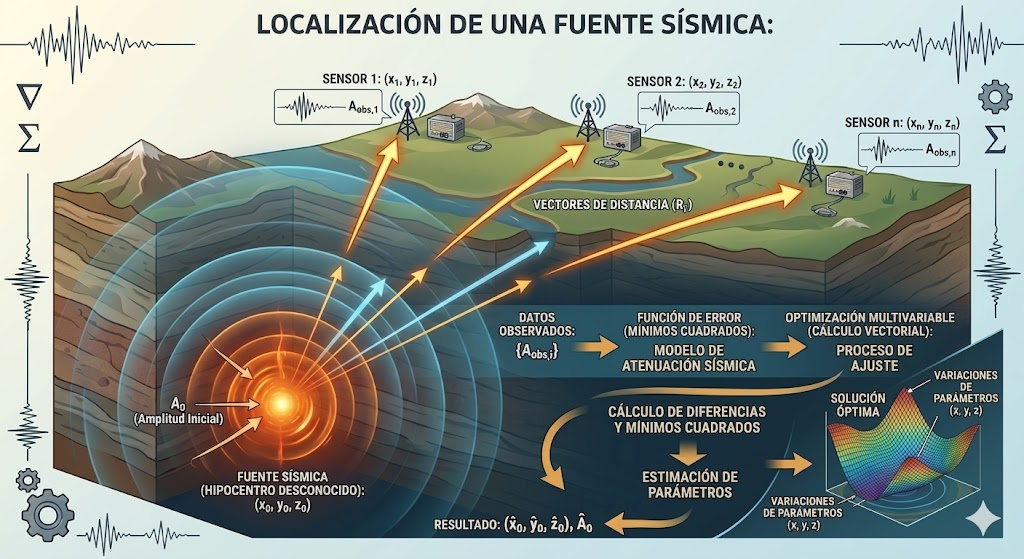
\includegraphics[width=0.7\textwidth]{Imagenes/LocalizacionFuenteSismica.png}
        \caption{Modelo de atenuación sísmica.}
    \end{figure}
\end{frame}
% Diapositiva 04
%Danilo
%===========================================
%   2. Qué es una fuente sísmica.
%===========================================



\begin{frame}{Modelo Geométrico de la Fuente Sísmica}
    \begin{figure}
        \centering
   
        \begin{tikzpicture}[x={(0.866cm,-0.5cm)}, y={(0.866cm,0.5cm)}, z={(0cm,1cm)}, scale=0.6, transform shape]
            
            % 1. Plano de la superficie terrestre (z = 0)
            \fill[gray!10, opacity=0.9] (-1,-1,0) -- (6,-1,0) -- (6,6,0) -- (-1,6,0) -- cycle;
            \draw[gray!40, thin, step=1] (-1,-1,0) grid (6,6,0);
            \node[anchor=west, text=gray!80!black] at (5.5, 5.5, 0) {Superficie Terrestre ($z=0$ km)};

            % 2. Ejes Coordenados
            \draw[thick,->, black!70] (0,0,0) -- (7,0,0) node[below right] {$x$};
            \draw[thick,->, black!70] (0,0,0) -- (0,7,0) node[above right] {$y$};
            \draw[thick,->, black!70] (0,0,-5) -- (0,0,3) node[above] {$z$};

            % 3. Fuente Sísmica (Hipocentro)
            \coordinate (Hipocentro) at (3, 3, -4);
            
            % Frentes de onda (representados como círculos concéntricos punteados)
            \foreach \r in {1, 2, 3} {
                \draw[orange, thick, dashed, opacity=0.7] (Hipocentro) circle (\r cm);
            }
            
            % Punto central de la fuente
            \fill[red] (Hipocentro) circle (3pt);
            \node[below, font=\bfseries, text=red!80!black, yshift=-3mm] at (Hipocentro) {Fuente: $(x_{\text{real}}, y_{\text{real}}, z_{\text{real}})$};

            % 4. Sensores en la superficie y vectores de distancia
            % Coordenadas de los sensores
            \coordinate (S1) at (1, 1, 0);
            \coordinate (S2) at (5, 2, 0);
            \coordinate (S3) at (2, 5, 0);

            % Bucle para dibujar cada sensor y su vector R
            \foreach \pos/\name in {S1/1, S2/2, S3/i} {
                % Dibujar el vector de distancia R primero para que quede debajo del sensor
                \draw[->, thick, blue!60] (Hipocentro) -- (\pos) node[midway, sloped, above, text=black] {$\vec{R}_{\name}$};
                
                % Dibujar el sensor (un pequeño triángulo/pirámide)
                \fill[black!80] (\pos) + (0,0,0.3) -- + (-0.2,-0.2,0) -- + (0.2,-0.2,0) -- cycle; 
                \node[above, font=\small, yshift=2mm] at (\pos) {Sensor $\name$};
            }

        \end{tikzpicture}
        % En las presentaciones, las descripciones cortas funcionan mejor
        \caption{Propagación de ondas y vectores de distancia en $\mathbb{R}^{3}$.}
        \label{fig:fuente_3d}
    \end{figure}
\end{frame}
%Danilo
\begin{frame}{Localización de la Fuente Sísmica}
    \begin{figure}
        \centering
        % Ajusta el ancho al 70% del tamaño de la diapositiva
        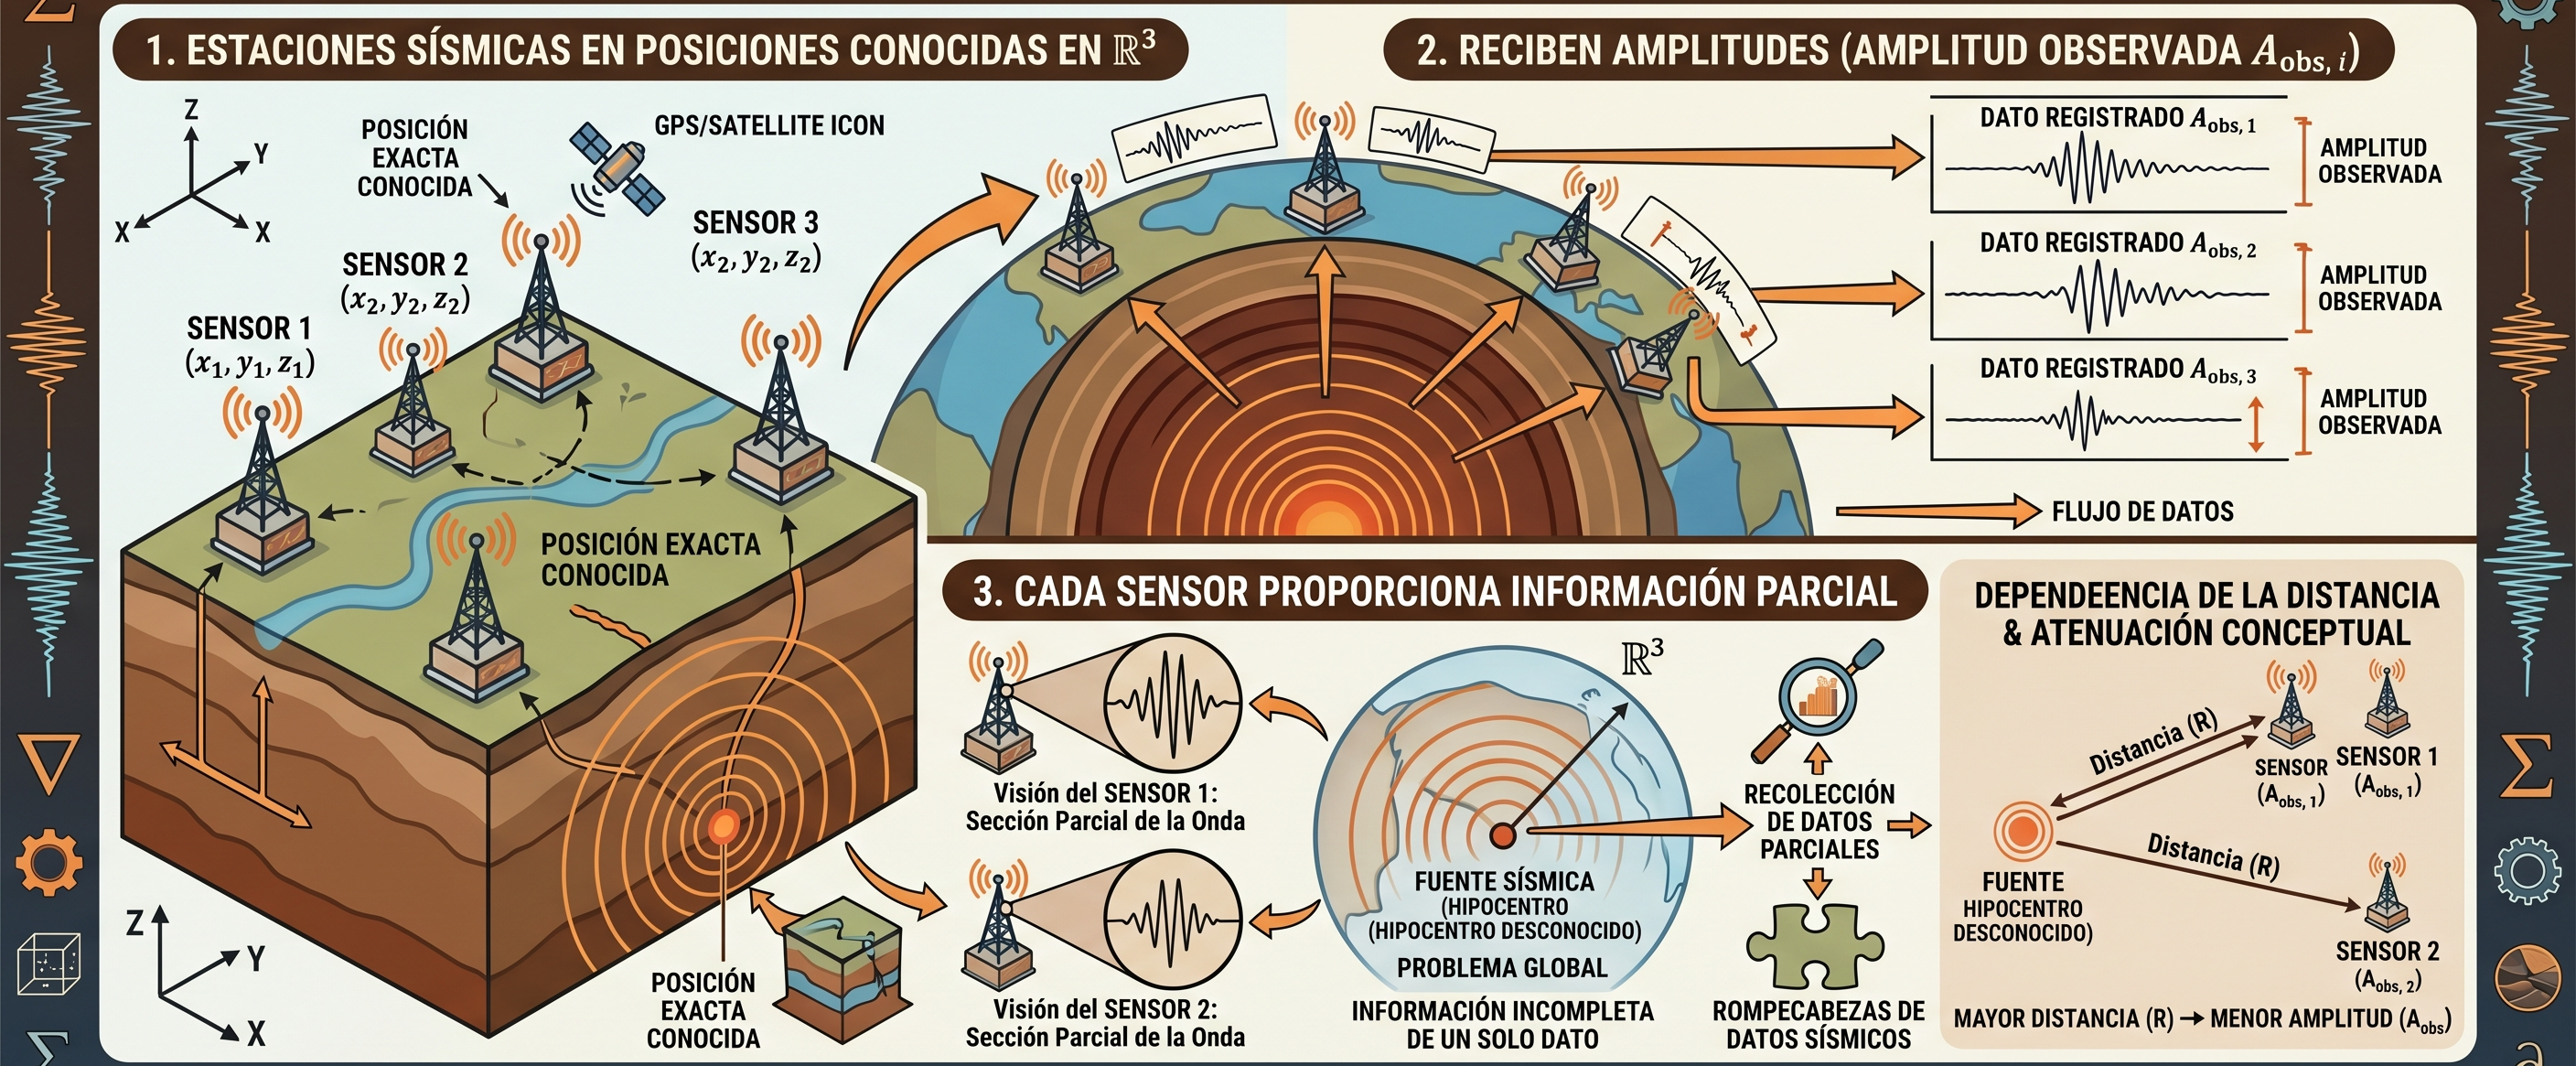
\includegraphics[width=0.7\textwidth]{Imagenes/RepresentacionSensores.png}
        \caption{Qué Representan los sensores en sismologia}
    \end{figure}
\end{frame}
% Diapositiva 06
% Kevin

%===========================================
%   4. Explicar la idea general del problema inverso
%   5.Diferenciar problema directo vs problema inverso
%   6.Explicar por qué se usa cálculo multivariado
%===========================================

\begin{frame}{Problema Directo vs Problema Inverso}

    \begin{center}
        \large \textbf{¿Qué información conocemos y qué buscamos?}
    \end{center}
    
    \vspace{0.1cm}
    
    \begin{columns}[T]
    
        %========================================
        % BLOQUE IZQUIERDO
        %========================================
        \column{0.48\textwidth}
        
        \begin{block}{Problema Directo}
            \begin{center}
                % Formalización matemática
                $ \mathbf{m} \longrightarrow \text{Datos} $
                
                \vspace{0.1cm}
                
                \begin{tikzpicture}[>=stealth, scale=0.75, transform shape]
                    % Fuente
                    \filldraw[red] (0,0) circle (0.18);
                    \node[below] at (0,-0.3) {\small Fuente Sísmica};
                    
                    % Sensores
                    \filldraw[blue] (3,1) circle (0.12);
                    \filldraw[blue] (3,0) circle (0.12);
                    \filldraw[blue] (3,-1) circle (0.12);
                    
                    \node[right] at (3,1) {\small S1};
                    \node[right] at (3,0) {\small S2};
                    \node[right] at (3,-1) {\small S3};
                    
                    % Ondas
                    \draw[->, thick] (0.2,0.1) -- (2.7,0.9);
                    \draw[->, thick] (0.2,0) -- (2.7,0);
                    \draw[->, thick] (0.2,-0.1) -- (2.7,-0.9);
                \end{tikzpicture}
                
                \vspace{0.1cm}
                
                \scriptsize
                Conocemos los parámetros $\mathbf{m} = [x_{\text{real}}, y_{\text{real}}, z_{\text{real}}, A_0]^T$ y calculamos las amplitudes esperadas.
            \end{center}
        \end{block}
    
        %========================================
        % BLOQUE DERECHO
        %========================================
        \column{0.48\textwidth}
        
        \begin{block}{Problema Inverso}
            \begin{center}
                % Formalización matemática
                $ \text{Datos} \longrightarrow \mathbf{m} $
                
                \vspace{0.1cm}
                
                \begin{tikzpicture}[>=stealth, scale=0.75, transform shape]
                    % Sensores
                    \filldraw[blue] (0,1) circle (0.12);
                    \filldraw[blue] (0,0) circle (0.12);
                    \filldraw[blue] (0,-1) circle (0.12);
                    
                    \node[left] at (0,1) {\small S1};
                    \node[left] at (0,0) {\small S2};
                    \node[left] at (0,-1) {\small S3};
                    
                    % Fuente desconocida
                    \filldraw[red] (3,0) circle (0.18);
                    \node[below] at (3,-0.3) {\small Fuente Estimada};
                    
                    % Flechas
                    \draw[->, thick] (0.2,0.9) -- (2.7,0.1);
                    \draw[->, thick] (0.2,0) -- (2.7,0);
                    \draw[->, thick] (0.2,-0.9) -- (2.7,-0.1);
                \end{tikzpicture}
                
                \vspace{0.1cm}
                
                \scriptsize
                A partir de las amplitudes observadas, estimamos el vector de parámetros $\mathbf{m} = [x_{\text{real}}, y_{\text{real}}, z_{\text{real}}, A_0]^T$.
            \end{center}
        \end{block}
    
    \end{columns}
    
    \vspace{0.2cm}
    
    \begin{center}
        \small \textit{“No observamos directamente la fuente; observamos únicamente sus efectos sobre los sensores.”}
    \end{center}
    
\end{frame}
% Diapositiva 07

% Kevin

%===========================================
% 7. Introducir el modelo de atenuación sísmica
% 8. Explicar qué representa la amplitud inicial A0
%===========================================



\begin{frame}{Modelo de Atenuación Sísmica}

    % PARTE SUPERIOR (CENTRO): La fórmula protagonista
    \begin{center}
        \LARGE % Hace que la fórmula destaque visualmente
        \[
        A_{pred,i} = A_0\frac{e^{-R_i}}{R_i}
        \]
    \end{center}
    
    \vspace{0.2cm}
    
    \begin{columns}[T]
    
        % PARTE IZQUIERDA: Explicación física visual
        \column{0.48\textwidth}
        \begin{center}
            
            % Se ajusta al 85% del ancho de esta columna
            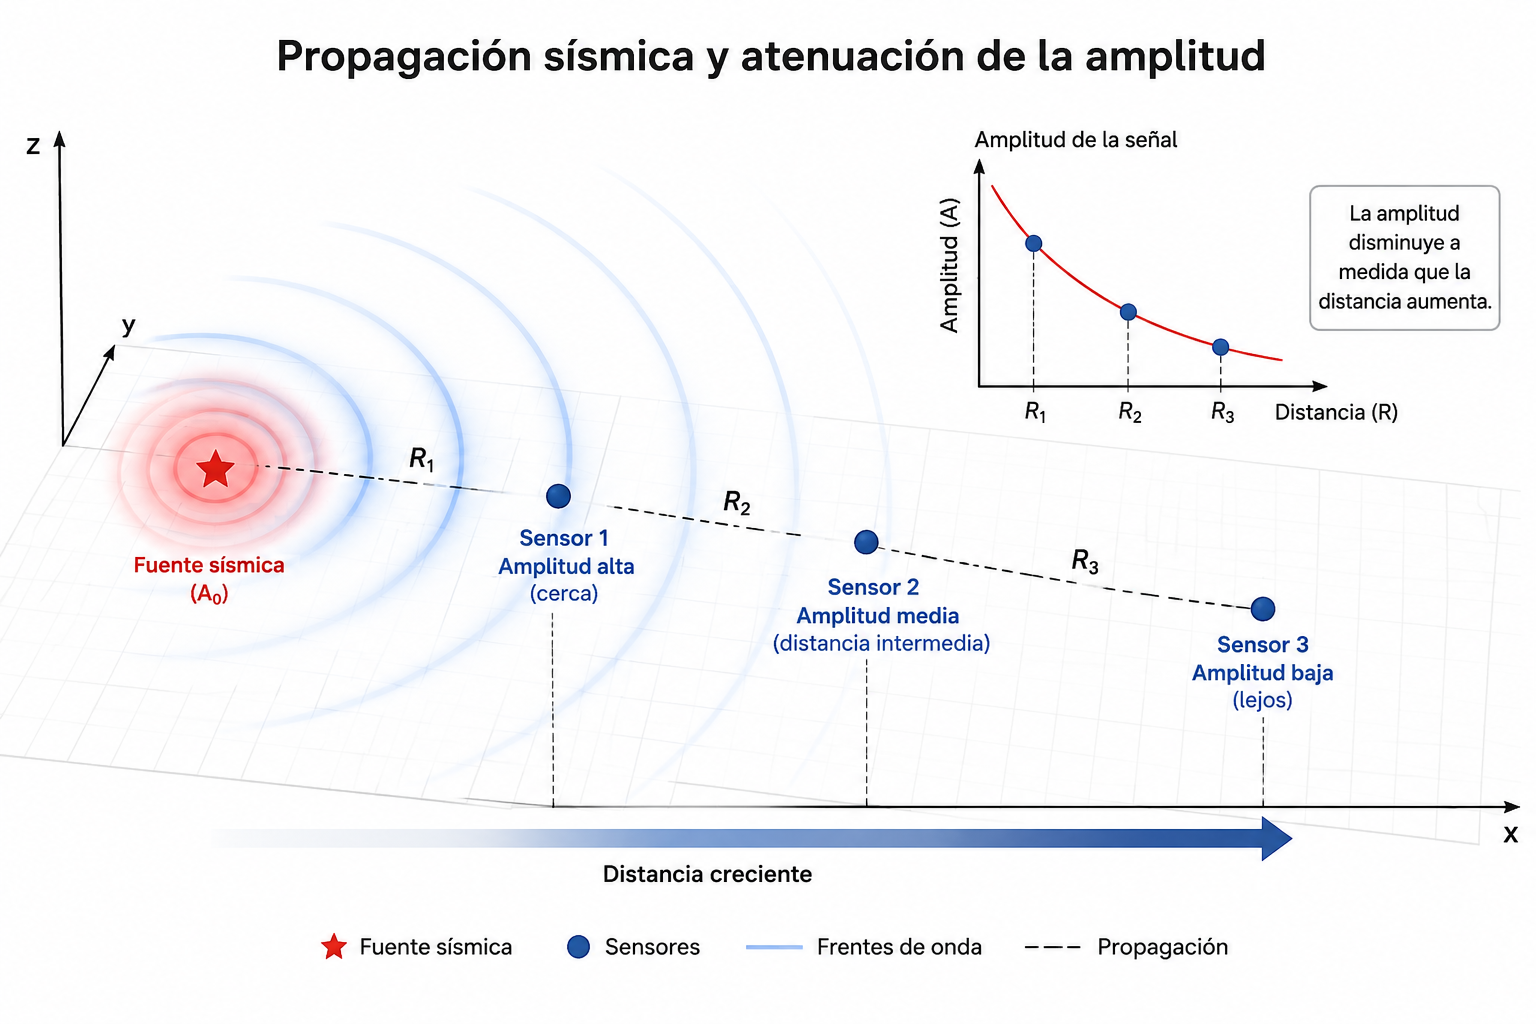
\includegraphics[width=0.80\textwidth]{Imagenes/PropagaciónSísmicaAtenuaciónAmplitud.png}
            
            \vspace{0.2cm}
            
            % Pequeño resumen del flujo por si Kevin necesita apoyarse al hablar
            \scriptsize
            Fuente Sísmica $\rightarrow$ Propagación $\rightarrow$ Pérdida de energía
        \end{center}
    
        % PARTE DERECHA: Significado de cada componente
        \column{0.48\textwidth}
        % Bajamos un poco el texto para que quede centrado respecto a la imagen
        \vspace{0.3cm} 
        
        \small
        \begin{itemize}
            \item $A_0$ : amplitud inicial de la fuente.
            \vspace{0.3cm} % Espacio extra entre items para mayor legibilidad
            
            \item $e^{-R_i}$ : atenuación de energía durante la propagación.
            \vspace{0.3cm}
            
            \item $\frac{1}{R_i}$ : dispersión geométrica de la onda.
            \vspace{0.3cm}
            
            \item $R_i$ : distancia entre la fuente y el sensor.
        \end{itemize}
        
    \end{columns}
    
    \vspace{0.4cm}
    
    % PARTE INFERIOR: Frase clave
    \begin{center}
        \textbf{
            La amplitud disminuye a medida que aumenta la \\ distancia entre la fuente y el sensor.
        }
    \end{center}

\end{frame}
\begin{frame}{Distancia Euclidiana en $\mathbb{R}^3$}

    \begin{columns}[c]

        %========================================
        % COLUMNA IZQUIERDA
        %========================================
        \column{0.50\textwidth}

        \begin{block}{Distancia Euclidiana}

            \centering
            \small

            \[
            R_i =
            \sqrt{
            (x_i-x)^2 +
            (y_i-y)^2 +
            (z_i-z)^2
            }
            \]

        \end{block}

        \vspace{0.25cm}

        \small
        \begin{itemize}

            \item $(x_i,y_i,z_i)$ : coordenadas conocidas del sensor $i$.

            \vspace{0.2cm}

            \item $(x,y,z)$ : posición estimada de la fuente sísmica.

            \vspace{0.2cm}

            \item $R_i$ : distancia tridimensional entre la fuente y el sensor.

        \end{itemize}

        \vspace{0.2cm}

        \begin{center}
            \small
            \textbf{
            Esta expresión mide la separación espacial entre dos puntos en $\mathbb{R}^3$.
            }
        \end{center}

        %========================================
        % COLUMNA DERECHA
        %========================================
        \column{0.46\textwidth}

        \begin{center}
            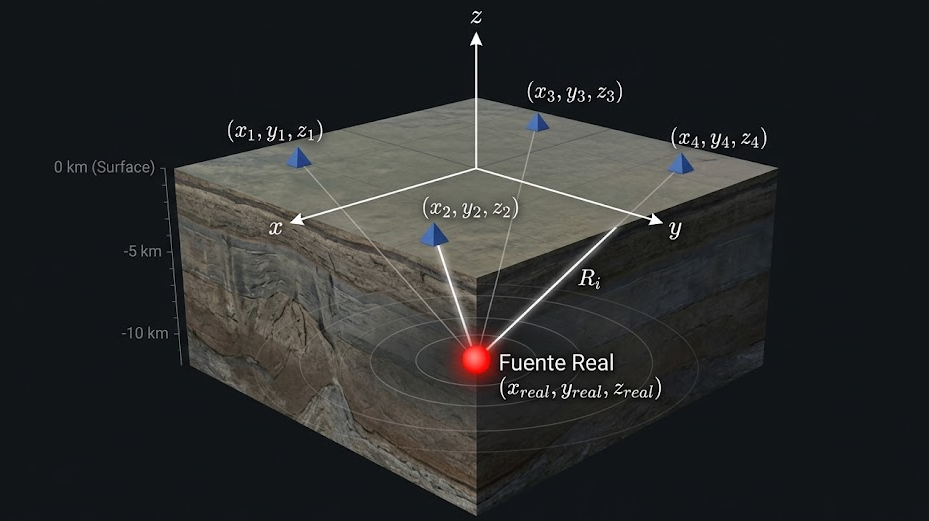
\includegraphics[width=\textwidth]{Imagenes/AtenuacioSismica.png}
        \end{center}

        \vspace{0.15cm}

        \begin{center}
            \tiny
            \textcolor{gray}{
            La geometría tridimensional permite determinar la distancia entre la fuente y cada sensor.
            }
        \end{center}

    \end{columns}

\end{frame}


%===========================================
%   2. Parte 2: Implementación y Resultados.
%===========================================
%Danilo
%===========================================
%   1.  Explicar que esta parte corresponde al problema directo
%   2.Presentar la fuente sísmica real simulada 
%   3.Explicar las coordenadas de la fuente
%   4.Explicar por qué z es negativo
%   5.Explicar la distancia euclidiana en R3
%============================================


\begin{frame}{Construcción del Problema Directo}

    % Usamos [c] para garantizar que todo el contenido flote exactamente en el centro vertical
    \begin{columns}[c]

        %========================================
        % COLUMNA IZQUIERDA: VISUALIZACIÓN
        %========================================
        \column{0.58\textwidth} % Le damos un poco más de ancho a la imagen

        \begin{center}
            % La imagen ahora domina este lado sin textos que compitan con ella
            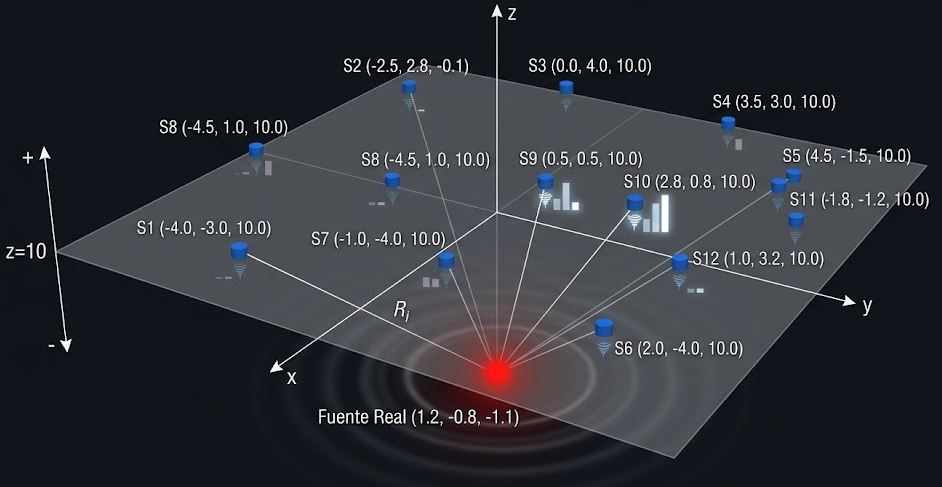
\includegraphics[width=\textwidth]{Imagenes/ProblemaDirecto3D.png}
        \end{center}

        %========================================
        % COLUMNA DERECHA: DATOS CLAVE
        %========================================
        \column{0.38\textwidth}

        %----------------------------------------
        % BLOQUE 1: ENTORNO
        %----------------------------------------
        % Convertimos el bullet point de R3 en un bloque elegante
        \begin{block}{Entorno del Modelo}
            \centering
            \vspace{0.2cm}
            Espacio tridimensional $\mathbb{R}^3$
            \vspace{0.2cm}
        \end{block}

        \vspace{0.8cm} % Un espacio grande para separar y usar bien el lienzo vacío

        %----------------------------------------
        % BLOQUE 2: PARÁMETROS REALES
        %----------------------------------------
        \begin{block}{Fuente Sísmica Real}
            \centering
            \vspace{0.2cm}
            
            \small
            \textbf{Coordenadas del Hipocentro:}
            \[
            (x_{\text{real}}, y_{\text{real}}, z_{\text{real}}) = (1.2, -0.8, -1.1)\ \text{km}
            \]
            \vspace{0.1cm}
        \end{block}

    \end{columns}

\end{frame}
%Danilo
%===========================================
%  6.explica su interpretación dentro del modelo.
%===========================================


\begin{frame}{Interpretación Geométrica}

    \begin{columns}[c]

        %========================================
        % COLUMNA IZQUIERDA
        %========================================
        \column{0.50\textwidth}

        \begin{block}{Relación entre distancia y amplitud}

            \small

            Mientras menor sea la distancia entre la fuente y un sensor, mayor será la amplitud registrada por dicho sensor.

            \vspace{0.2cm}

            Por eso, la distancia $R_i$ se convierte en una variable fundamental dentro del modelo matemático.

        \end{block}

        \vspace{0.25cm}

        \begin{block}{Idea física}

            \small

            La señal se atenúa al propagarse, de modo que los sensores más alejados registran amplitudes menores.

        \end{block}

        \vspace{0.15cm}

        \begin{center}
            \small
            \textbf{
            La geometría espacial controla el comportamiento de las amplitudes sísmicas.
            }
        \end{center}

        %========================================
        % COLUMNA DERECHA
        %========================================
        \column{0.46\textwidth}

        \begin{center}
            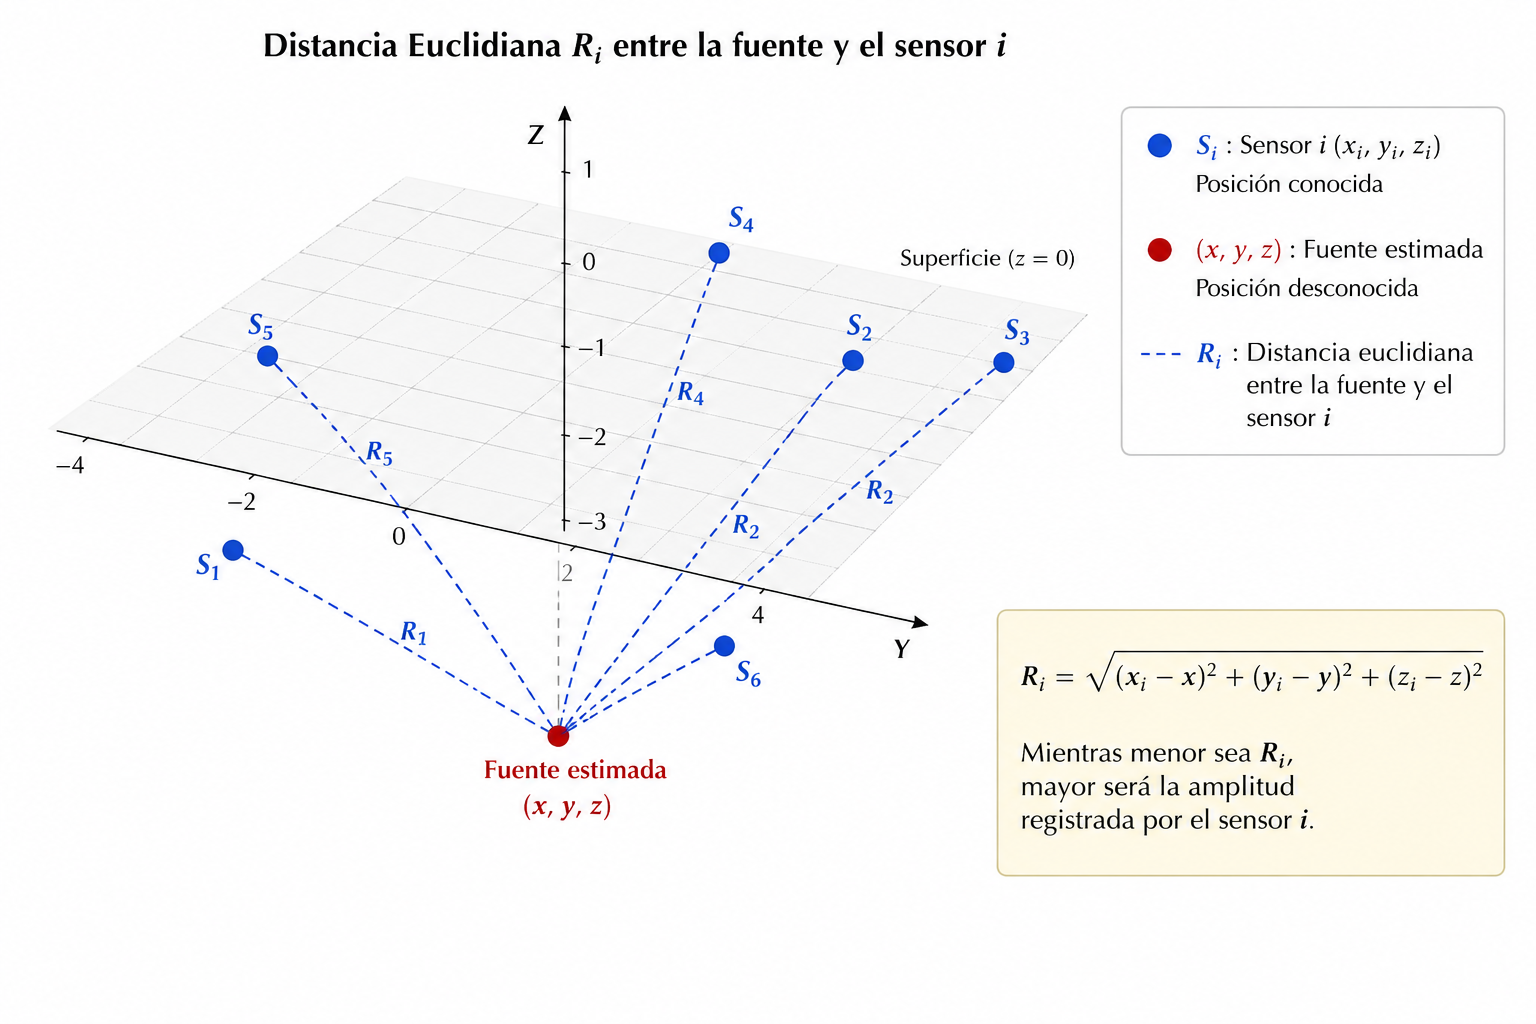
\includegraphics[width=\textwidth]{Imagenes/DistanciaEuclidiana3D.png}
        \end{center}

        \vspace{0.15cm}

        \begin{center}
            \tiny
            \textcolor{gray}{
            La posición de la fuente modifica las distancias $R_i$ y, en consecuencia, las amplitudes predichas por el modelo.
            }
        \end{center}

    \end{columns}

\end{frame}
% Diapositiva 11

% Danilo
%============================================
% 8. Explicar cómo se distribuyeron los sensores
% 9. Explicar por qué se utilizaron 12 sensores
% 10.Mostrar la distribución espacial de sensores
%============================================


\begin{frame}{Distribución de Sensores}
    \begin{figure}
        \centering
        % Ajusta el ancho al 70% del tamaño de la diapositiva
        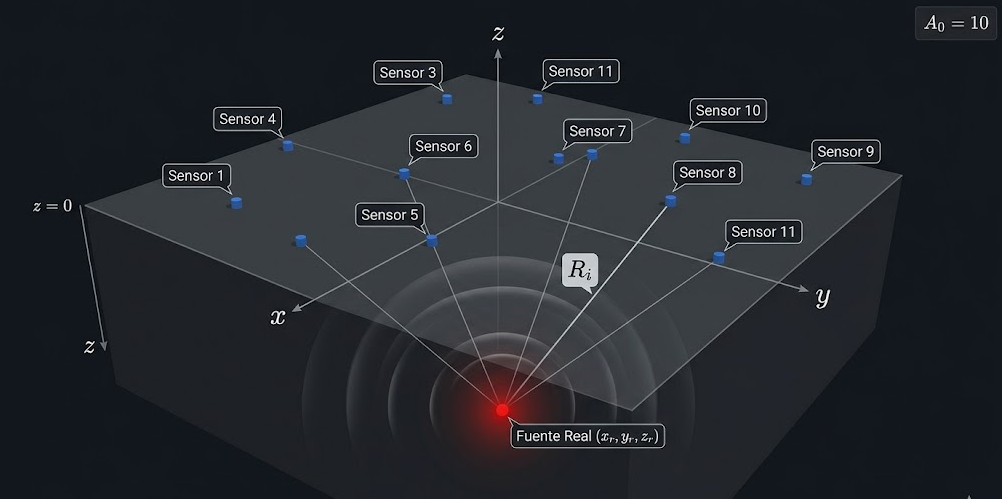
\includegraphics[width=0.7\textwidth]{Imagenes/Distribucio_sensores.png}
        \caption{Modelo de Distribución de Sensores.}
    \end{figure}
\end{frame}
%Luchando los dias 
%============================================
%  Explicar Los daots que se usaran para este promblema 
%=============================================

\begin{frame}{Generación de Datos Simulados}

    \begin{columns}[c]

        %========================================
        % COLUMNA IZQUIERDA: Tabla de Sensores
        %========================================
        \column{0.50\textwidth}
        \begin{block}{Ubicación de Sensores ($S_i$)}
            \centering
            \scriptsize 
            \begin{tabular}{@{}lccc@{}}
                \toprule
                \textbf{Sensor} & \textbf{$x_i$} & \textbf{$y_i$} & \textbf{$z_i$} \\ \midrule
                S1 & -4.0 & -3.0 & 0.2 \\
                S2 & -2.5 & 2.8 & -0.1 \\
                S3 & 0.0 & 4.0 & 0.1 \\
                S4 & 3.5 & 3.0 & -0.2 \\
                S5 & 4.5 & -1.5 & 0.0 \\
                S6 & 2.0 & -4.0 & 0.3 \\
                S7 & -1.0 & -4.5 & -0.1 \\
                S8 & -4.5 & 1.0 & 0.2 \\
                S9 & 0.5 & 0.5 & 0.0 \\
                S10 & 2.8 & 0.8 & -0.3 \\
                S11 & -1.8 & -1.2 & 0.1 \\
                S12 & 1.0 & 3.2 & 0.2 \\ \bottomrule
            \end{tabular}
        \end{block}

        %========================================
        % COLUMNA DERECHA: Resumen Ejecutivo
        %========================================
        \column{0.45\textwidth}

        \begin{block}{Configuración de Red}
            \small
            \begin{itemize}
                \item \textbf{Muestra:} $n = 12$ sensores.
                \item \textbf{Espacio:} Distribución tridimensional.
            \end{itemize}
        \end{block}

        \vspace{0.4cm}

        \begin{block}{Estrategia de Simulación}
            \scriptsize
            \begin{itemize}
                \item Cobertura multidireccional.
                \item Estabilidad del problema inverso.
                \item Generación de amplitudes ideales.
            \end{itemize}
        \end{block}

        \vspace{0.6cm}
        
        \begin{center}
            \tiny \textcolor{gray}{Red optimizada para localización robusta de la fuente.}
        \end{center}

    \end{columns}

\end{frame}
% Diapositiva 13

% Luis 
%============================================
% 11. Explicar Procedimientos para agregar ruido Gaussiano
%=============================================

\begin{frame}{Cálculo Paso a Paso: Distancia Euclidiana ($R_1$)}

    \begin{columns}[T]
        %========================================
        % COLUMNA IZQUIERDA: Contexto (Reducida al 30%)
        %========================================
        \column{0.30\textwidth}
        \begin{block}{Datos del Sensor 1}
            \scriptsize
            \textbf{S1:} $(-4.0, -3.0, 0.2)$ km \\
            \textbf{Fuente:} $(x_{\text{real}}, y_{\text{real}}, z_{\text{real}}) = (1.2, -0.8, -1.1)$ km
        \end{block}

        \vspace{0.4cm}

        \begin{block}{Nota Técnica}
            \tiny
            Sustitución de parámetros en la métrica euclidiana para determinar el radio de propagación.
        \end{block}

        %========================================
        % COLUMNA DERECHA: Operación (Ampliada al 68%)
        %========================================
        \column{0.68\textwidth}
        \begin{exampleblock}{Procedimiento Detallado}
            \centering
            \footnotesize % Tamaño ideal para que la raíz no se corte
            \begin{align*}
                R_1 &= \sqrt{(x_1 - x_{\text{real}})^2 + (y_1 - y_{\text{real}})^2 + (z_1 - z_{\text{real}})^2} \\[0.15cm]
                R_1 &= \sqrt{(-4.0 - 1.2)^2 + (-3.0 - (-0.8))^2 + (0.2 - (-1.1))^2} \\[0.15cm]
                R_1 &= \sqrt{(-5.2)^2 + (-3.0 + 0.8)^2 + (0.2 + 1.1)^2} \\[0.15cm]
                R_1 &= \sqrt{(-5.2)^2 + (-2.2)^2 + (1.3)^2} \\[0.15cm]
                R_1 &= \sqrt{27.04 + 4.84 + 1.69} \\[0.15cm]
                R_1 &= \sqrt{33.57} \implies \mathbf{R_1 \approx 5.794}
            \end{align*}
        \end{exampleblock}
    \end{columns}

    \vspace{0.3cm}
    \begin{center}
        \tiny \textcolor{gray}{Cálculo fundamental para la posterior aplicación del modelo de atenuación.}
    \end{center}

\end{frame}


% Diapositiva 14

% Luis
%============================================
% 12. Explicar ese valor mínimo y máximo de la tabla 
%=============================================

\begin{frame}{Resultados: Distancias Calculadas}

    \begin{columns}[c]

        %========================================
        % COLUMNA IZQUIERDA: Tabla de Resultados
        %========================================
        \column{0.58\textwidth}
        \begin{block}{Distancia a cada Sensor ($R_i$ [km])}
            \centering
            \scriptsize 
            \begin{tabular}{@{}lcccc@{}}
                \toprule
            \textbf{Sensor} & \textbf{$x_i$ [km]} & \textbf{$y_i$ [km]} & \textbf{$z_i$ [km]} & \textbf{$R_i$ [km]} \\ \midrule
                S1  & -4.0 & -3.0 &  0.2 & 5.7940 \\
                S2  & -2.5 &  2.8 & -0.1 & 5.2583 \\
                S3  &  0.0 &  4.0 &  0.1 & 5.0912 \\
                S4  &  3.5 &  3.0 & -0.2 & 4.5321 \\
                S5  &  4.5 & -1.5 &  0.0 & 3.5482 \\
                S6  &  2.0 & -4.0 &  0.3 & 3.5833 \\
                S7  & -1.0 & -4.5 & -0.1 & 4.4193 \\
                S8  & -4.5 &  1.0 &  0.2 & 6.1172 \\
                S9  &  0.5 &  0.5 &  0.0 & 1.8412 \\
                S10 &  2.8 &  0.8 & -0.3 & 2.4000 \\
                S11 & -1.8 & -1.2 &  0.1 & 3.2558 \\
                S12 &  1.0 &  3.2 &  0.2 & 4.2107 \\ \bottomrule
            \end{tabular}
        \end{block}

        %========================================
        % COLUMNA DERECHA: Análisis Crítico
        %========================================
        \column{0.38\textwidth}

        \begin{block}{Análisis de la Red}
            \scriptsize
            Resultados tras aplicar la métrica euclidiana desde la fuente real a cada nodo.
        \end{block}

        \vspace{0.4cm}

        \begin{block}{Valores Críticos}
            \scriptsize
            \begin{itemize}
                \item \textbf{Mínimo:} S9 ($R_9 \approx 1.84$ km) \\
                \vspace{0.1cm}
                $\rightarrow$ \textit{Mayor amplitud esperada.}
                
                \vspace{0.4cm}
                
                \item \textbf{Máximo:} S8 ($R_8 \approx 6.12$ km) \\
                \vspace{0.1cm}
                $\rightarrow$ \textit{Mayor atenuación (pérdida).}
            \end{itemize}
        \end{block}

    \end{columns}

\end{frame}
% Diapositiva 15

% Luchando los dias

%============================================
% 13. cómo se usaron dentro de la simulación la formula de las amplitudes ideales.
% 14. Explicar el valor usado para A0
%=============================================

\begin{frame}{Generación de Amplitudes Simuladas}

    \begin{columns}[T] % Alineación superior para evitar desplazamientos
        
        %========================================
        % COLUMNA IZQUIERDA: VISUALIZACIÓN
        %========================================
        \column{0.55\textwidth}
        \begin{center}
            % Reducimos un poco la imagen para ganar espacio vertical
            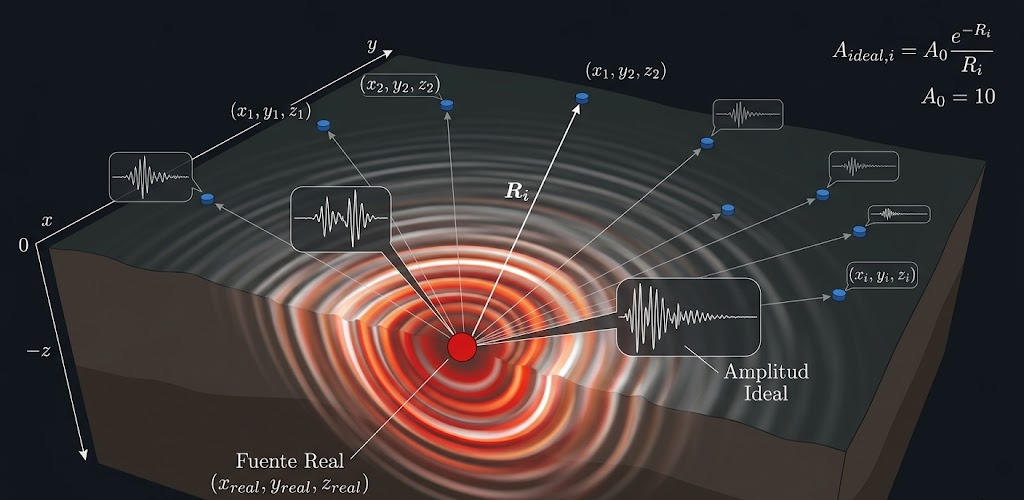
\includegraphics[width=0.85\textwidth]{Imagenes/Amplitudes_Ideales.png}
            
            \vspace{0.1cm}
            \tiny \textcolor{gray}{
                Distribución de sensores y fuente sísmica simulada.
            }
        \end{center}

        %========================================
        % COLUMNA DERECHA: MODELO Y SÍNTESIS
        %========================================
        \column{0.42\textwidth}
        
        \begin{block}{Modelo de Simulación}
            \centering
            \small
            $A_0 = 10$
            \vspace{0.1cm}
            \[
            A_{ideal,i} = A_0 \frac{e^{-R_i}}{R_i}
            \]
        \end{block}

        \vspace{0.2cm} % Espacio reducido entre bloques

        \begin{block}{Flujo de Información}
            \scriptsize
            \begin{itemize}
                \item \textbf{Cálculo:} Amplitudes obtenidas mediante distancias $R_i$.
                \item \textbf{Transición:} Datos de entrada para el problema inverso.
            \end{itemize}
        \end{block}

    \end{columns}

    \vspace{0.3cm} % Espacio controlado para la frase final

    \begin{center}
        \footnotesize
        \textbf{El modelo directo construye el escenario que el algoritmo inverso deberá resolver.}
    \end{center}

\end{frame}

% Diapositiva 16

% Luchando los dias
%============================================
% 15. Explicar procedimiento de las amplitudes ideales
%=============================================

\begin{frame}{Cálculo de Amplitudes Ideales ($A_{ideal}$)}

    \begin{columns}[T]
        %========================================
        % COLUMNA IZQUIERDA: Tabla de Datos Ri
        %========================================
        \column{0.48\textwidth}
        \begin{block}{Entradas: Coordenadas y Distancia}
            \centering
            \scriptsize 
            \begin{tabular}{@{}lcccc@{}}
                \toprule
                \textbf{Sens.} & \textbf{$x_i$} & \textbf{$y_i$} & \textbf{$z_i$} & \textbf{$R_i$} \\ \midrule
                S1  & -4.0 & -3.0 &  0.2 & 5.7940 \\
                S2  & -2.5 &  2.8 & -0.1 & 5.2583 \\
                S3  &  0.0 &  4.0 &  0.1 & 5.0912 \\
                S4  &  3.5 &  3.0 & -0.2 & 4.5321 \\
                S5  &  4.5 & -1.5 &  0.0 & 3.5482 \\
                S6  &  2.0 & -4.0 &  0.3 & 3.5833 \\
                S7  & -1.0 & -4.5 & -0.1 & 4.4193 \\
                S8  & -4.5 &  1.0 &  0.2 & 6.1172 \\
                S9  &  0.5 &  0.5 &  0.0 & 1.8412 \\
                S10 &  2.8 &  0.8 & -0.3 & 2.4000 \\
                S11 & -1.8 & -1.2 &  0.1 & 3.2558 \\
                S12 &  1.0 &  3.2 &  0.2 & 4.2107 \\ \bottomrule
            \end{tabular}
        \end{block}

        %========================================
        % COLUMNA DERECHA: Procedimiento Paso a Paso
        %========================================
        \column{0.48\textwidth}
        \begin{exampleblock}{Procedimiento ($S_1$)}
            \centering
            \footnotesize
            % Se redujo el salto de línea de 0.3cm a 0.1cm para ahorrar espacio vertical
            \begin{align*}
                A_{ideal,i} &= A_0 \frac{e^{-R_i}}{R_i} \\[0.1cm]
                A_{ideal,1} &= 10 \frac{e^{-5.7940}}{5.7940} \\[0.1cm]
                A_{ideal,1} &\approx 10 \frac{0.003045}{5.7940} \\[0.1cm]
                \mathbf{A_{ideal,1}} &\approx \mathbf{0.005257}
            \end{align*}
        \end{exampleblock}

        \vspace{0.1cm} % Reducido para acercar la nota al bloque superior

        \begin{block}{Nota del Modelo}
            \scriptsize
            Cálculo determinista basado en el decaimiento exponencial y dispersión geométrica.
        \end{block}
    \end{columns}

\end{frame}
\begin{frame}{Resultados: Tabulación de Amplitudes Ideales}

    \begin{columns}[T]
        %========================================
        % COLUMNA IZQUIERDA: Tabla de Datos
        %========================================
        \column{0.50\textwidth}
        \begin{block}{Consolidado de Resultados}
            \centering
            \scriptsize 
            \begin{tabular}{@{}lcc@{}}
                \toprule
                \textbf{Sensor} & \textbf{Distancia $R_i$} & \textbf{Amplitud $A_{ideal}$} \\ \midrule
                S1  & 5.7940 & 0.005257 \\
                S2  & 5.2583 & 0.009897 \\
                S3  & 5.0912 & 0.012081 \\
                S4  & 4.5321 & 0.023737 \\
                S5  & 3.5482 & 0.081097 \\
                S6  & 3.5833 & 0.077538 \\
                S7  & 4.4193 & 0.027251 \\
                S8  & 6.1172 & 0.003604 \\
                % Fila resaltada únicamente con negrita para evitar errores de compilación
                \textbf{S9} & \textbf{1.8412} & \textbf{0.861547} \\
                S10 & 2.4000 & 0.377991 \\
                S11 & 3.2558 & 0.118410 \\
                S12 & 4.2107 & 0.035234 \\ \bottomrule
            \end{tabular}
        \end{block}

        %========================================
        % COLUMNA DERECHA: Análisis Resumido
        %========================================
        \column{0.45\textwidth}
        \vspace{0.4cm}
        
        \begin{block}{Observaciones Clave}
            \scriptsize
            \begin{itemize}
                \item \textbf{Sensor Crítico (S9):} Menor distancia $\rightarrow$ Mayor amplitud registrada.
                \vspace{0.4cm}
                \item \textbf{Atenuación:} El decaimiento es consistente con el modelo exponencial.
                \vspace{0.4cm}
                \item \textbf{Uniformidad:} Los resultados servirán de base para el algoritmo de inversión.
            \end{itemize}
        \end{block}

        \vspace{0.6cm}
        \begin{center}
            \tiny \textit{Amplitudes calculadas mediante $A_{ideal} = A_0 \frac{e^{-R}}{R}$ con $A_0=10$.}
        \end{center}
    \end{columns}

\end{frame}
% Luchando los dias
%===========================================
% 16. Incorporación de ruido gaussiano moderado y Explicar Procedimientos para agregar ruido Gaussiano 
%===========================================

\begin{frame}{Incorporación de Ruido Gaussiano}

    \begin{columns}[T]
        %========================================
        % COLUMNA IZQUIERDA: Justificación Física
        %========================================
        \column{0.48\textwidth}
        \begin{block}{¿Por qué añadir ruido?}
            \scriptsize
            Para simular condiciones reales de medición:
            \begin{itemize}
                \item Errores instrumentales de los sensores.
                \item Variaciones e irregularidades del medio.
                \item Pequeñas perturbaciones externas.
            \end{itemize}
        \end{block}

        \vspace{0.2cm}

        \begin{block}{Naturaleza del Ruido ($\epsilon_i$)}
            \scriptsize
            \begin{itemize}
                \item \textbf{Distribución Normal:} Media cero ($\mu = 0$).
                \item \textbf{Imparcialidad:} No introduce tendencias; puede aumentar o disminuir el valor ideal.
            \end{itemize}
        \end{block}

        %========================================
        % COLUMNA DERECHA: Formulación Matemática
        %========================================
        \column{0.48\textwidth}
        \begin{exampleblock}{Modelado Matemático}
            \centering
            \footnotesize
            \textbf{Variación moderada (5\%)}
            \[ \text{Factor} = 0.05 \]
            
            \textbf{Desviación Estándar ($\sigma_i$)}
            \[ \sigma_i = 0.05 \cdot A_{ideal,i} \]
            
            \textbf{Generación de Ruido}
            \[ \epsilon_i \sim N(0, \sigma_i) \]
            
            \textbf{Amplitud Observada}
            \[ \mathbf{A_{obs,i} = A_{ideal,i} + \epsilon_i} \]
        \end{exampleblock}
    \end{columns}

    \vspace{0.4cm}
    \begin{center}
        \footnotesize 
        \textbf{El ruido transforma una simulación perfecta en un escenario de datos realistas.}
    \end{center}

\end{frame}
% Luchando los dias
%===========================================
% 17. Explicar aplicacion de ruido gaussiano y resultados obtenidos
%===========================================


\begin{frame}{Tabulación: Amplitudes Observadas ($A_{obs}$)}

    \begin{columns}[T]
        %========================================
        % COLUMNA IZQUIERDA: Tabla de Datos con Ruido
        %========================================
        \column{0.65\textwidth}
        \begin{block}{Cálculo: $A_{obs,i} = A_{ideal,i} + \epsilon_i$}
            \centering
            \scriptsize 
            \begin{tabular}{@{}lcccc@{}}
                \toprule
                \textbf{Sensor} & \textbf{$R_i$} & \textbf{$A_{ideal}$} & \textbf{$\epsilon_i$ (5\%)} & \textbf{$A_{obs}$} \\ \midrule
                S1  & 5.7940 & 0.005257 & +0.000263 & \textbf{0.005520} \\
                S2  & 5.2583 & 0.009897 & -0.000495 & \textbf{0.009402} \\
                S3  & 5.0912 & 0.012081 & +0.000604 & \textbf{0.012685} \\
                S4  & 4.5321 & 0.023737 & -0.001187 & \textbf{0.022550} \\
                S5  & 3.5482 & 0.081097 & +0.004055 & \textbf{0.085152} \\
                S6  & 3.5833 & 0.077538 & -0.003877 & \textbf{0.073661} \\
                S7  & 4.4193 & 0.027251 & +0.001363 & \textbf{0.028614} \\
                S8  & 6.1172 & 0.003604 & -0.000180 & \textbf{0.003424} \\
                \textbf{S9} & \textbf{1.8412} & \textbf{0.861547} & \textbf{+0.043077} & \textbf{0.904624} \\
                S10 & 2.4000 & 0.377991 & -0.018900 & \textbf{0.359091} \\
                S11 & 3.2558 & 0.118410 & +0.005921 & \textbf{0.124331} \\
                S12 & 4.2107 & 0.035234 & -0.001762 & \textbf{0.033472} \\ \bottomrule
            \end{tabular}
        \end{block}

        %========================================
        % COLUMNA DERECHA: Análisis Técnico
        %========================================
        \column{0.32\textwidth}
        \vspace{0.8cm}
        
        \begin{block}{Datos de Entrada}
            \scriptsize
            Estas amplitudes perturbadas constituyen el set de datos real para la inversión sísmica.
        \end{block}

        \vspace{0.4cm}

        \begin{block}{Impacto del Ruido}
            \scriptsize
            La variación del 5\% simula la incertidumbre instrumental sin comprometer la tendencia física del modelo.
        \end{block}
    \end{columns}

\end{frame}

%===========================================
%   3. Parte 3: Problema Inverso y Comparación de Resultados.
%===========================================
% Diapositiva 20
% Kevin
%=============================================
% 1. Explicar qué significa comparar amplitudes observadas y predichas.
%=============================================

\begin{frame}{Comparación de Amplitudes: Lógica Inversa}

    \begin{columns}[T]
        %========================================
        % COLUMNA IZQUIERDA: VISUALIZACIÓN
        %========================================
        \column{0.52\textwidth}
        \begin{center}
            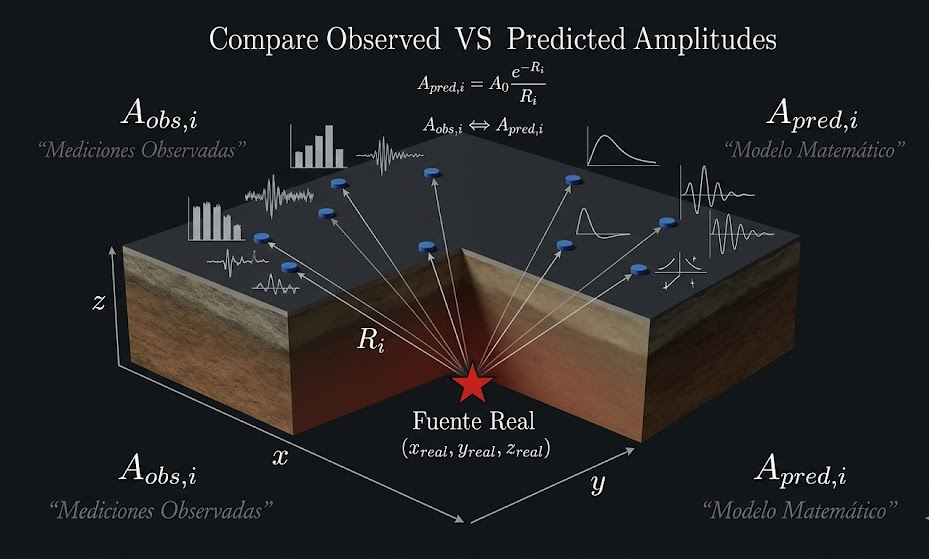
\includegraphics[width=0.95\textwidth]{Imagenes/AmplitudesObservadasPredichas.png}
        \end{center}

        \vspace{-0.2cm}
        \begin{center}
            \tiny \textcolor{gray}{
            Contraste entre mediciones ruidosas y el modelo teórico.
            }
        \end{center}

        %========================================
        % COLUMNA DERECHA: FUNDAMENTO TÉCNICO
        %========================================
        \column{0.44\textwidth}
        
        \begin{block}{Fundamento Inverso}
            \scriptsize 
            \begin{itemize}
                \item \textbf{Diferencial:} Contraste entre registradas ($A_{obs}$) y teóricas ($A_{pred}$).
                \vspace{0.2cm}
                \item \textbf{Criterio:} El ajuste óptimo indica proximidad a la fuente real.
                \vspace{0.2cm}
                \item \textbf{Convergencia:} 
                \[ A_{pred} \approx A_{obs} \implies \text{Proximidad} \]
            \end{itemize}
        \end{block}

        \begin{exampleblock}{Modelo Matemático}
            \centering
            \footnotesize
            \[ A_{pred,i} = A_0 \frac{e^{-R_i}}{R_i} \]
        \end{exampleblock}

    \end{columns}

    \vspace{0.3cm} 
    \begin{center}
        \footnotesize 
        \textbf{Minimizar la discrepancia entre la física y la medición.}
    \end{center}

\end{frame}
% Diapositiva 21

% Kevin
%=============================================
% 2. Explicar por qué se construye una función de error
% 3. Explicar qué significa minimizar el error
% 4. Explicar por qué se usan mínimos cuadrados
% 5. Introducir la función de error
%=============================================

\begin{frame}{Construcción de la Función de Error}

    \begin{columns}[T]
        %========================================
        % COLUMNA IZQUIERDA: VISUALIZACIÓN
        %========================================
        \column{0.50\textwidth}
        \begin{center}
            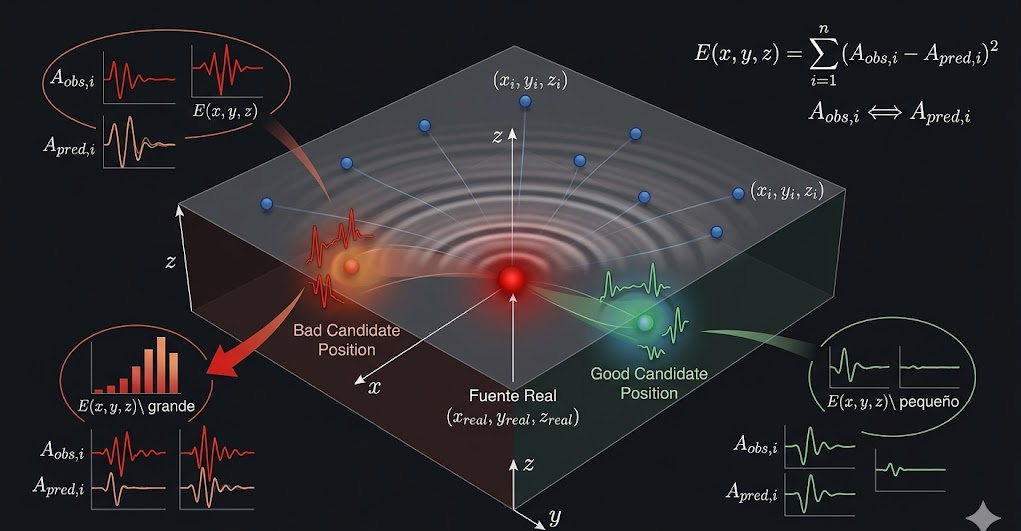
\includegraphics[width=0.95\textwidth]{Imagenes/FuncionErroryMinimizacion.png}
        \end{center}

        \vspace{-0.2cm}
        \begin{center}
            \tiny \textcolor{gray}{
            Superficie matemática del error acumulado de la red.
            }
        \end{center}

        %========================================
        % COLUMNA DERECHA: MÉTRICA Y JUSTIFICACIÓN
        %========================================
        \column{0.46\textwidth}

        \begin{block}{Métrica de Ajuste Global}
            \centering
            \small
            \[ E(x,y,z) = \sum_{i=1}^{n} \left( A_{obs,i} - A_{pred,i} \right)^2 \]
        \end{block}

        \vspace{0.1cm}

        \begin{block}{¿Por qué Mínimos Cuadrados?}
            \scriptsize
            \begin{itemize}
                \item \textbf{Sin Cancelación:} Evita que errores positivos y negativos se anulen entre sí.
                \item \textbf{Penalización:} Magnifica fuertemente las discrepancias más grandes.
            \end{itemize}
        \end{block}

        \vspace{0.1cm}

        \begin{block}{Restricción del Modelo}
            \scriptsize
            \textbf{Optimización espacial:} La amplitud inicial $A_0 = 10$ se mantiene fija. La búsqueda se realiza únicamente sobre $(x,y,z)$.
        \end{block}

    \end{columns}

    \vspace{0.3cm}
    \begin{center}
        \footnotesize 
        \textbf{La función mide qué tan distante es la respuesta teórica frente a la realidad medida.}
    \end{center}

\end{frame}
% Diapositiva 22
% David

%=============================================
% 6. Explicar que el mínimo representa la mejor estimación
%=============================================
\begin{frame}{Optimización: Interpretación del Mínimo Global}

    \begin{columns}[T]
        %========================================
        % COLUMNA IZQUIERDA: El Objetivo Matemático
        %========================================
        \column{0.48\textwidth}
        \begin{block}{Criterio de Optimización}
            \scriptsize
            Determinación del punto óptimo en el espacio tridimensional mediante la minimización del error global:
            \vspace{0.3cm}
            \[
            (x^*, y^*, z^*) = \arg\min E(x,y,z)
            \]
            \vspace{0.2cm}
        \end{block}

        \vspace{0.2cm}

        \begin{block}{Validación del Modelo}
            \scriptsize
            Un valor residual bajo de $E(x,y,z)$ certifica que las coordenadas evaluadas reproducen con alta fidelidad las amplitudes medidas.
        \end{block}

        %========================================
        % COLUMNA DERECHA: ¿Qué significa realmente?
        %========================================
        \column{0.48\textwidth}
        \begin{exampleblock}{Significado Físico-Matemático}
            \scriptsize
            El punto mínimo de la función representa:
            \begin{itemize}
                \item \textbf{Ajuste Óptimo:} La menor discrepancia físicamente alcanzable respecto a la red de sensores.
                \vspace{0.3cm}
                \item \textbf{Consistencia:} Región espacial donde las predicciones teóricas convergen con los datos de campo.
            \end{itemize}
        \end{exampleblock}
    \end{columns}

    \vspace{0.5cm}

    \begin{center}
        \footnotesize
        \textbf{"   El mínimo no es solo un valor numérico decreciente; es la posición espacial que mejor explica el evento sísmico real."}
    \end{center}

\end{frame}
% Diapositiva 23
% David
%=============================================
% . Mostrar los datos utilizados para la estimación 
%=============================================
\begin{frame}{Datos Utilizados para la Estimación}

    \begin{columns}[T]
        %========================================
        % COLUMNA IZQUIERDA: Tabla de Sensores (Inputs)
        %========================================
        \column{0.55\textwidth}
        \begin{block}{Entradas: Coordenadas y Observaciones}
            \centering
            \scriptsize 
            \begin{tabular}{@{}lcccc@{}}
                \toprule
                \textbf{Sensor} & \textbf{$x_i$ [km]} & \textbf{$y_i$ [km]} & \textbf{$z_i$ [km]} & \textbf{$Az_i$ obs.} \\ \midrule
                S1  & -4.0 & -3.0 &  0.2 & 0.005219 \\
                S2  & -2.5 &  2.8 & -0.1 & 0.009811 \\
                S3  &  0.0 &  4.0 &  0.1 & 0.012014 \\
                S4  &  3.5 &  3.0 & -0.2 & 0.024570 \\
                S5  &  4.5 & -1.5 &  0.0 & 0.080580 \\
                S6  &  2.0 & -4.0 &  0.3 & 0.071733 \\
                S7  & -1.0 & -4.5 & -0.1 & 0.027704 \\
                S8  & -4.5 &  1.0 &  0.2 & 0.003556 \\
                \textbf{S9}  & \textbf{0.5} & \textbf{0.5} & \textbf{0.0} & \textbf{0.852201} \\
                S10 &  2.8 &  0.8 & -0.3 & 0.380182 \\
                S11 & -1.8 & -1.2 &  0.1 & 0.119785 \\
                S12 &  1.0 &  3.2 &  0.2 & 0.037284 \\ \bottomrule
            \end{tabular}
        \end{block}

        %========================================
        % COLUMNA DERECHA: Parámetros Clave
        %========================================
        \column{0.42\textwidth}
        \vspace{0.5cm}

        \begin{block}{Parámetros del Problema Inverso}
            \centering
            \scriptsize
            \begin{tabular}{@{}ll@{}}
                \toprule
                \textbf{Elemento} & \textbf{Valor [km]} \\ \midrule
                Fuente real $(x_{\text{real}},\ y_{\text{real}},\ z_{\text{real}})$ & $(1.2, -0.8, -1.1)$ \\ \vspace{0.1cm}
                Amplitud inicial & $A_0 = 10$ \\ \vspace{0.1cm}
                Red instrumental & $12$ sensores \\ \vspace{0.1cm}
                Dato de ajuste & $Az_i$ observado \\ \bottomrule
            \end{tabular}
        \end{block}

        \vspace{0.5cm}
        
        \begin{block}{Objetivo}
            \scriptsize
            Utilizar el set de datos $Az_i$ para que el algoritmo recupere las coordenadas de la fuente real ocultas en la simulación.
        \end{block}

    \end{columns}

\end{frame}
\begin{frame}{Estrategia de Búsqueda y Optimización}

    \begin{columns}[T]
        %========================================
        % COLUMNA IZQUIERDA: Algoritmos
        %========================================
        \column{0.45\textwidth}
        
        \begin{block}{1. Nelder-Mead (Principal)}
            \scriptsize
            \begin{itemize}
                \item Algoritmo numérico iterativo.
                \item Busca el mínimo de la función de error sin usar derivadas.
            \end{itemize}
        \end{block}

        \vspace{0.3cm}

        \begin{block}{2. Búsqueda por Grilla (Soporte)}
            \scriptsize
            \begin{itemize}
                \item Exploración espacial estructurada.
                \item Útil para visualización conceptual, no como optimizador final.
            \end{itemize}
        \end{block}

        %========================================
        % COLUMNA DERECHA: Rangos
        %========================================
        \column{0.50\textwidth}
        
        \begin{block}{Acotación del Dominio ($x, y, z$)}
            \centering
            \scriptsize
            \vspace{0.1cm}
            \begin{tabular}{@{}lcc@{}}
                \toprule
                \textbf{Eje} & \textbf{Rango} & \textbf{Justificación Física} \\ \midrule
                $x$ & $[-5, 5]$ & Cobertura horizontal de la red. \\ \vspace{0.1cm}
                $y$ & $[-5, 5]$ & Cobertura horizontal de la red. \\ \vspace{0.1cm}
                $z$ & $[-3, 1]$ & Profundidad del hipocentro. \\ \bottomrule
            \end{tabular}
        \end{block}

        \vspace{0.4cm}
        \begin{center}
            \footnotesize
            \textbf{Limitar el dominio asegura la convergencia numérica.}
        \end{center}
    \end{columns}

\end{frame}
% El mono jojoi
%=============================================
% 7. Explicar el método de optimización principal: Nelder-Mead
%=============================================


\begin{frame}{Método de Optimización Principal: Nelder-Mead}

    \begin{columns}[T]
        %========================================
        % COLUMNA IZQUIERDA: LÓGICA Y ECUACIONES
        %========================================
        \column{0.48\textwidth} % Ligeramente más ancha para evitar saltos de línea
        
        \begin{block}{Dinámica Geométrica}
            \scriptsize
            \begin{itemize}
                \item \textbf{Mecanismo:} Despliega un simplex (poliedro de 4 vértices) en el espacio 3D.
                \item \textbf{Adaptación:} Se refleja, expande o contrae buscando la pendiente de menor error.
            \end{itemize}
        \end{block}

        \begin{exampleblock}{Operaciones de Búsqueda}
            \scriptsize
            \begin{itemize}
                \item \textbf{Reflexión:} Proyección al mejor ajuste: $x_r = x_c + \alpha(x_c - x_{\text{peor}})$
                \item \textbf{Expansión:} Se acelera si el nuevo error es menor: $E(x_r) < E_{\text{mejor}}$.
                \item \textbf{Contracción:} Se encoge si el error aumenta.
            \end{itemize}
        \end{exampleblock}

        \begin{block}{Robustez del Método}
            \scriptsize
            Alta tolerancia para absorber las perturbaciones del ruido gaussiano (5\%).
        \end{block}

        %========================================
        % COLUMNA DERECHA: IMAGEN CONCEPTUAL
        %========================================
        \column{0.48\textwidth}
        \vspace{0.2cm}
        \begin{center}
            % Ajusta el nombre del archivo según cómo lo hayas guardado
            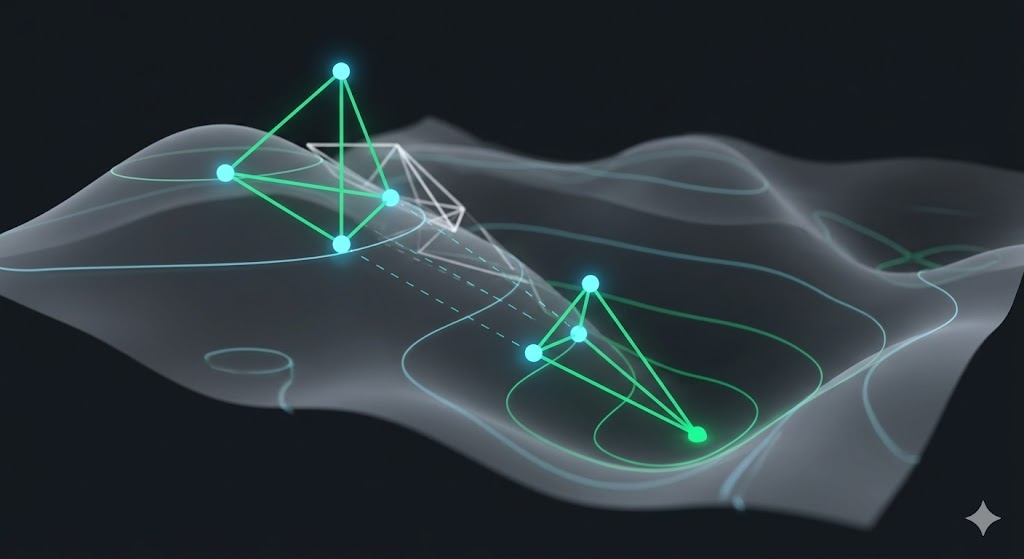
\includegraphics[width=\textwidth]{Imagenes/NelderMeadVisual.png}
        \end{center}
        
        \vspace{-0.3cm}
        \begin{center}
            \tiny \textcolor{gray}{
            Representación conceptual del simplex iterando sobre la topografía del error.
            }
        \end{center}

    \end{columns}

\end{frame}
% Le mono jojoi
%=============================================
% 8.1. Explicar que también se utilizó búsqueda por grilla como apoyo visual
%=============================================

\begin{frame}{Algoritmo Numérico: Búsqueda por Grilla}

    \begin{columns}[T]
        
        %=======================================================
        % COLUMNA IZQUIERDA: BLOQUE VERDE (Pseudocódigo)
        %=======================================================
        \column{0.63\textwidth}
        \begin{exampleblock}{Lógica del Algoritmo de Exploración}
            \scriptsize % Letra pequeña para que las fórmulas largas quepan sin problema
            \textbf{Inicialización:} $E_{\text{min}} \leftarrow \infty$ \\[0.15cm]
            \begin{tabbing}
                \quad \= \quad \= \quad \= \quad \= \kill
                $\mathbf{para}$ cada $x$ dentro del rango sugerido $\mathbf{hacer}$ \\
                \> $\mathbf{para}$ cada $y$ dentro del rango sugerido $\mathbf{hacer}$ \\
                \> \> $\mathbf{para}$ cada $z$ dentro del rango sugerido $\mathbf{hacer}$ \\[0.1cm]
                \> \> \> 1. $R_i = \sqrt{(x_i - x)^2 + (y_i - y)^2 + (z_i - z)^2}$ \\
                \> \> \> 2. $A_{pred,i} = A_0 \frac{e^{-R_i}}{R_i}$ \\
                \> \> \> 3. $E(x,y,z) = \sum_{i=1}^{n} (A_{obs,i} - A_{pred,i})^2$ \\[0.1cm]
                \> \> \> $\mathbf{si}$ $E(x,y,z) < E_{\text{min}}$ $\mathbf{entonces}$ \\
                \> \> \> \> $E_{\text{min}} \leftarrow E(x,y,z)$ \\
                \> \> \> \> $\text{mejor\_punto} \leftarrow (x,y,z)$
            \end{tabbing}
        \end{exampleblock}

        %=======================================================
        % COLUMNA DERECHA: BLOQUES AZULES APILADOS
        %=======================================================
        \column{0.34\textwidth}
        
        \begin{block}{Procesamiento Espacial}
            \scriptsize
            \begin{itemize}
                \item \textbf{Discretización:} Evaluación en mallas tridimensionales.
                \vspace{0.1cm}
                \item \textbf{Métrica:} Validación simultánea en la red de sensores.
            \end{itemize}
        \end{block}

        \vspace{0.3cm}

        \begin{block}{Soporte Conceptual}
            \scriptsize
            \begin{itemize}
                \item \textbf{Topografía:} Mapea la superficie de error.
                \vspace{0.1cm}
                \item \textbf{Garantía:} Valida visualmente la existencia del mínimo global.
            \end{itemize}
        \end{block}

    \end{columns}

    \vspace{0.3cm}
    \begin{center}
        \footnotesize
        \textbf{La estructura iterativa asegura un rastreo exhaustivo del hipocentro.}
    \end{center}

\end{frame}
\begin{frame}{Ejemplo Numérico del Procedimiento de Cálculo}

    \begin{columns}[T]
        %========================================
        % COLUMNA IZQUIERDA: LOS PASOS LÓGICOS
        %========================================
        \column{0.46\textwidth}
        \begin{block}{Mecánica de Evaluación}
            \scriptsize
            Para cada punto candidato $(x,y,z)$, el algoritmo ejecuta tres pasos secuenciales por cada sensor:
            \begin{enumerate}
                \item \textbf{Geometría:} Calcula la distancia euclidiana 3D al sensor.
                \item \textbf{Física:} Evalúa la atenuación teórica ($A_{pred}$).
                \item \textbf{Estadística:} Obtiene el residuo individual.
            \end{enumerate}
        \end{block}

        \vspace{0.1cm}

        \begin{block}{Acumulación del Costo}
            \scriptsize
            Este procedimiento matemático se repite de forma idéntica para los 12 sensores de la red. La sumatoria de estos residuos cuadrados es la que define el error global $E(x,y,z)$.
        \end{block}

        %========================================
        % COLUMNA DERECHA: LA CORRIDA EN FRÍO REAL (S9)
        %========================================
        \column{0.50\textwidth}
        \begin{exampleblock}{Traza de Ejecución Real (Sensor 9)}
            \tiny
            Evaluación en el punto estimado: $(1.2001, -0.7765, -1.1381)$ \\
            Datos de $S_9$: Coordenadas $(0.5, 0.5, 0.0)$ y $Az_{obs} = 0.852201$
            
            \vspace{0.15cm}
            \textbf{Paso 1: Distancia Euclidiana ($R_9$)}
            \[ R_9 = \sqrt{(0.5 - 1.2001)^2 + (0.5 - (-0.7765))^2 + (0.0 - (-1.1381))^2} \]
            \[ R_9 = \sqrt{(-0.7001)^2 + (1.2765)^2 + (1.1381)^2} \approx 1.8479 \]

            \vspace{0.1cm}
            \textbf{Paso 2: Amplitud Predicha ($A_{pred,9}$)}
            \[ A_{pred,9} = 10 \cdot \frac{e^{-1.8479}}{1.8479} \approx 0.852651 \]

            \vspace{0.1cm}
            \textbf{Paso 3: Residuo Individual}
            \[ \text{Residuo} = A_{obs,9} - A_{pred,9} \]
            \[ \text{Residuo} = 0.852201 - 0.852651 = -0.000450 \]
        \end{exampleblock}
    \end{columns}

\end{frame}
\begin{frame}{Dataset Instrumental: Coordenadas y Amplitudes}
    \begin{block}{Tabla 1: Datos de entrada para la Función de Error}
        \centering
        \scriptsize
        \begin{tabular}{@{}lcccc@{}}
            \toprule
            \textbf{Sensor} & \textbf{$x_i$} & \textbf{$y_i$} & \textbf{$z_i$} & \textbf{$Az_i$ observado} \\ \midrule
            S1  & -4.0 & -3.0 &  0.2 & 0.005219 \\
            S2  & -2.5 &  2.8 & -0.1 & 0.009811 \\
            S3  &  0.0 &  4.0 &  0.1 & 0.012014 \\
            S4  &  3.5 &  3.0 & -0.2 & 0.024570 \\
            S5  &  4.5 & -1.5 &  0.0 & 0.080580 \\
            S6  &  2.0 & -4.0 &  0.3 & 0.071733 \\
            S7  & -1.0 & -4.5 & -0.1 & 0.027704 \\
            S8  & -4.5 &  1.0 &  0.2 & 0.003556 \\
            \textbf{\textcolor{blue}{S9}}  & \textbf{\textcolor{blue}{0.5}} & \textbf{\textcolor{blue}{0.5}} & \textbf{\textcolor{blue}{0.0}} & \textbf{\textcolor{blue}{0.852685}} \\
            S10 &  2.8 &  0.8 & -0.3 & 0.380182 \\
            S11 & -1.8 & -1.2 &  0.1 & 0.119785 \\
            S12 &  1.0 &  3.2 &  0.2 & 0.037284 \\ \bottomrule
        \end{tabular}
    \end{block}
    \vspace{0.2cm}
    \begin{center}
        \tiny \textcolor{gray}{*Nota: Los datos de S9 resaltados son los utilizados en el ejemplo numérico de la siguiente diapositiva.}
    \end{center}
\end{frame}
\begin{frame}{Resultados de la Estimación y Comparación}

    \begin{columns}[T]
        %========================================
        % COLUMNA IZQUIERDA: MÉTRICAS Y GRÁFICA
        %========================================
        \column{0.48\textwidth}
        \begin{block}{Convergencia Numérica}
            \scriptsize
            El algoritmo Nelder-Mead convergió a un residuo óptimo:
            \[ E_{min} \approx 2.8592 \times 10^{-5} \]
        \end{block}

        \vspace{0.1cm}
        
        \begin{center}
            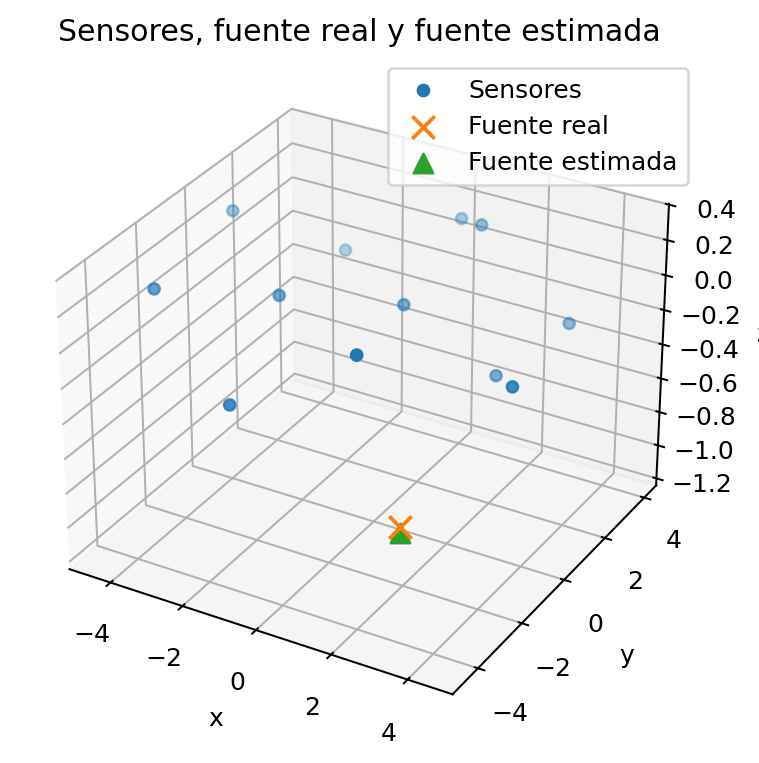
\includegraphics[width=0.9\textwidth]{Imagenes/EstimacionValidacion.png}
            \\ \tiny \textcolor{gray}{Comparativa visual: Fuente Real vs Estimada.}
        \end{center}

        %========================================
        % COLUMNA DERECHA: TABLA COMPARATIVA
        %========================================
        \column{0.48\textwidth}
        \begin{block}{Comparación Definitiva}
            \centering
            \scriptsize
            \begin{tabular}{@{}lccc@{}}
                \toprule
                \textbf{Par.} & \textbf{Real} & \textbf{Est.} & \textbf{Dif.} \\ \midrule
                $x$ & 1.2000 & 1.2001 & 0.0001 \\
                $y$ & -0.8000 & -0.7765 & 0.0235 \\
                $z$ & -1.1000 & -1.1381 & 0.0381 \\ \bottomrule
            \end{tabular}
            
            \vspace{0.2cm}
            \textbf{Distancia neta:} \\
            $\Delta \approx 0.0448$ unidades
        \end{block}

        \begin{block}{Interpretación Física}
            \scriptsize
            Las desviaciones en $y$ y $z$ son consistentes con la perturbación gaussiana del 5\% aplicada al modelo.
        \end{block}
    \end{columns}

\end{frame}
\begin{frame}{Revisión de Residuales por Sensor}

    \begin{columns}[T]
        %========================================
        % COLUMNA IZQUIERDA: TABLA EXACTA
        %========================================
        \column{0.48\textwidth}
        \begin{block}{Tabla de Residuales (Datos Reales)}
            \centering
            \tiny % Usamos tiny para que quepan las 12 filas
            \begin{tabular}{@{}lcccc@{}}
                \toprule
                \textbf{Sen.} & \textbf{Obs.} & \textbf{Pred.} & \textbf{Resid.} & \textbf{|Res|} \\ \midrule
                S1  & 0.005219 & 0.005149 & 0.000070 & 0.000070 \\
                S2  & 0.009811 & 0.009999 & -0.000188 & 0.000188 \\
                S3  & 0.012014 & 0.012270 & -0.000256 & 0.000256 \\
                S4  & 0.024570 & 0.024087 & 0.000483 & 0.000483 \\
                S5  & 0.080580 & 0.079390 & 0.001190 & 0.001190 \\
                S6  & 0.071733 & 0.074057 & -0.002324 & 0.002324 \\
                S7  & 0.027704 & 0.026317 & 0.001387 & 0.001387 \\
                S8  & 0.003556 & 0.003598 & -0.000042 & 0.000042 \\
                S9  & 0.852201 & 0.852651 & -0.000450 & 0.000450 \\
                S10 & 0.380182 & 0.379389 & 0.000793 & 0.000793 \\
                S11 & 0.119785 & 0.115769 & 0.004016 & 0.004016 \\
                S12 & 0.037284 & 0.035687 & 0.001597 & 0.001597 \\ \bottomrule
            \end{tabular}
        \end{block}

        %========================================
        % COLUMNA DERECHA: IMAGEN Y CONCLUSIÓN
        %========================================
        \column{0.48\textwidth}
        \vspace{0.5cm}
        \begin{center}
            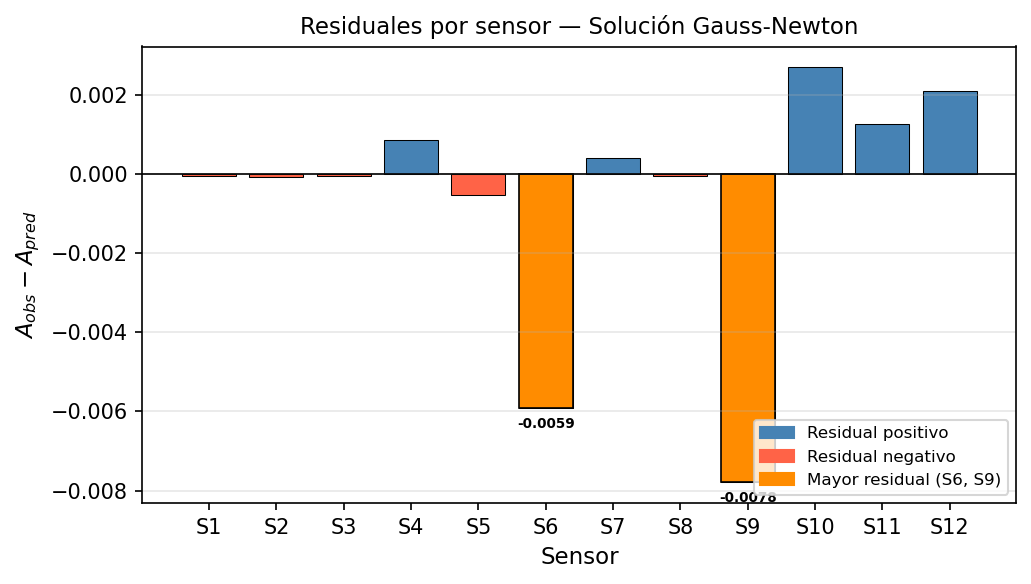
\includegraphics[width=\textwidth]{Imagenes/ResidualSensor.png}
            \\[0.2cm]
            \tiny \textcolor{gray}{Distribución de residuales por sensor.}
        \end{center}
        
        \vspace{-0.9cm}
        \begin{block}{Interpretación}
            \scriptsize
            La baja magnitud de los residuos (del orden de $10^{-3}$ a $10^{-4}$) confirma que el modelo propuesto tiene un ajuste preciso sobre la red de 12 sensores simulados.
        \end{block}
    \end{columns}

\end{frame}

%===========================================
%   4. Parte 4: Visualización y Mapas de Calor.
%===========================================
% Diapositiva 31
%  El mono 
%=============================================
% Puntos 1, 2, 3: Por qué E(x,y,z,A0) no se puede visualizar completa,
% qué significa fijar z, y cortes bidimensionales.
%=============================================

\section{Visualización y Mapas de Calor}

\begin{frame}{Visualización de $E(x,y,z,A_0)$: El Problema Dimensional}

    \begin{columns}[T]

        \column{0.48\textwidth}

        \begin{block}{¿Por qué no se puede graficar directamente?}
            \scriptsize
            La función de error depende \textbf{simultáneamente} de cuatro parámetros:
            \[
                E = E(x,\, y,\, z,\, A_0)
            \]
            \begin{itemize}
                \item Una gráfica convencional solo admite \textbf{dos dimensiones}.
                \item Representar $E$ completa requeriría un espacio \textbf{5D}.
                \item Por tanto, la visualización directa \textbf{no es posible}.
            \end{itemize}
            \vspace{0.15cm}
            \textbf{Estrategia:} Se fijan $z$ y $A_0$ en sus valores óptimos y se analiza:
            \[
                E(x, y)\Big|_{z = z_{\text{real}},\; A_0 = A_0^*}
            \]
            Esto reduce el problema a \textbf{dos variables} visualizables.
        \end{block}

        \column{0.48\textwidth}

        \begin{block}{¿Qué representa cada corte?}
            \scriptsize
            \begin{itemize}
                \item Cada corte es una \textbf{fotografía} de la función de error a una profundidad fija.
                \vspace{0.15cm}
                \item Permite observar la \textbf{distribución espacial} del error en el plano $(x, y)$.
                \vspace{0.15cm}
                \item Variando $z$ se obtiene una \textbf{secuencia de cortes} que describe el comportamiento volumétrico de $E$.
            \end{itemize}
        \end{block}

        \vspace{0.2cm}

        \begin{block}{Idea Central}
            \centering
            \scriptsize
            Fijar $z$ y $A_0$ convierte un problema \textbf{5D} en uno \textbf{2D} visualizable.
        \end{block}

    \end{columns}

    \vspace{0.2cm}
    \begin{center}
        \footnotesize
        \textbf{Los cortes bidimensionales son la herramienta clave para explorar $E(x,y,z,A_0)$.}
    \end{center}

\end{frame}
% Alejandro
%=============================================
% Tabla de parámetros clave del proyecto
%=============================================

\begin{frame}{Parámetros del Modelo: Datos de Referencia}

    \begin{columns}[T]

        \column{0.50\textwidth}

        \begin{block}{Parámetros de la Simulación}
            \centering
            \scriptsize
            \begin{tabular}{@{}lp{3.2cm}@{}}
                \toprule
                \textbf{Elemento} & \textbf{Valor [km]} \\ \midrule
                Fuente real $(x_{\text{real}},\ y_{\text{real}},\ z_{\text{real}})$ & $(1.2,\ {-0.8},\ {-1.1})$ \\[0.2cm]
                Fuente estimada & $(1.200,\ {-0.777},\ {-1.138})$ \\[0.2cm]
                Amplitud inicial $A_0$ & $10$ \\[0.2cm]
                Número de sensores & $12$ \\[0.2cm]
                Función evaluada & $E = \sum_{i=1}^{n}(A_{obs,i} - A_{pred,i})^2$ \\
                \bottomrule
            \end{tabular}
        \end{block}

        \column{0.46\textwidth}

        \begin{block}{Rangos de Búsqueda en la Grilla}
            \centering
            \scriptsize
            \begin{tabular}{@{}lcc@{}}
                \toprule
                \textbf{Var.} & \textbf{Rango [km]} & \textbf{Justificación} \\ \midrule
                $x$ & $[-5,\ 5]$ & Cubre la red de sensores \\[0.2cm]
                $y$ & $[-5,\ 5]$ & Cubre la red de sensores \\[0.2cm]
                $z$ & $[-3,\ 1]$ & Incluye prof. sísmicas \\
                \bottomrule
            \end{tabular}
        \end{block}

        \vspace{0.2cm}

        \begin{exampleblock}{Cortes de Profundidad Analizados [km]}
            \centering
            \scriptsize
            \begin{tabular}{@{}lp{3.5cm}@{}}
                \toprule
                \textbf{Corte} & \textbf{Significado} \\ \midrule
                $z = -0.50$ & Plano menos profundo que la fuente \\[0.1cm]
                $z = -1.10$ & Profundidad real de la fuente \\[0.1cm]
                $z = -1.14$ & Profundidad estimada por optimización \\[0.1cm]
                $z = -1.70$ & Plano más profundo, análisis comparativo \\
                \bottomrule
            \end{tabular}
        \end{exampleblock}

    \end{columns}

    \vspace{0.1cm}
    \begin{center}
        \tiny \textcolor{gray}{*Todas las coordenadas están expresadas en kilómetros (km).}
    \end{center}

\end{frame}
% Diapositiva 33, 34 → El mono | Diapositiva 35 → David | Diapositiva 36 → Danilo

%  El mono (frames 33 y 34) — David (frame 35) — Danilo (frame 36) 
%=============================================
% Puntos 4-10: Mapas de calor, curvas de nivel,
% regiones de bajo error, cortes de profundidad.
%=============================================

% -----------------------------------------------
% FRAME 30a: z = -0.50
% -----------------------------------------------
\begin{frame}{Mapa de Calor: Corte en $z = -0.50$ km — Plano Superficial}

    \begin{columns}[T]

        \column{0.55\textwidth}

        \begin{block}{Corte en $z = -0.50$ km}
            \centering
            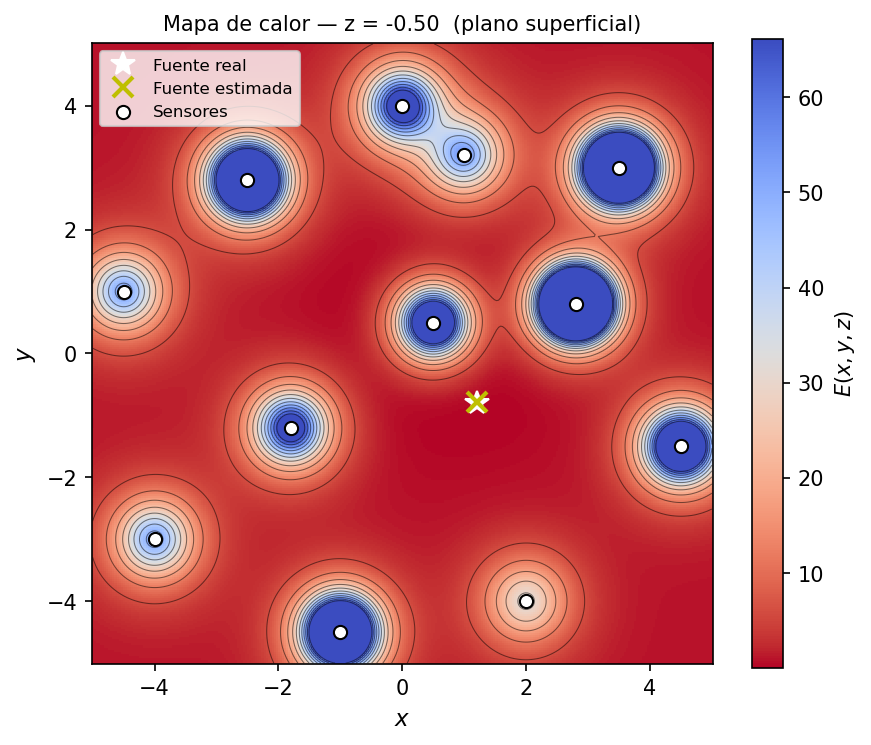
\includegraphics[width=0.95\textwidth]{Imagenes/corte_z_050.png}
        \end{block}

        \column{0.41\textwidth}

        \begin{block}{Interpretación}
            \scriptsize
            \begin{itemize}
                \item Este plano está \textbf{por encima} de la fuente real $z_{\text{real}} = -1.10$ km.
                \vspace{0.1cm}
                \item El error es \textbf{alto y disperso}: no hay una región mínima clara.
                \vspace{0.1cm}
                \item Las curvas de nivel no convergen a un punto definido.
            \end{itemize}
        \end{block}

        \vspace{0.2cm}

        \begin{exampleblock}{¿Qué nos dice?}
            \scriptsize
            A esta profundidad el modelo \textbf{no logra reproducir} las amplitudes observadas, confirmando que la fuente no está aquí.
        \end{exampleblock}

    \end{columns}

    \vspace{0.1cm}
    \begin{center}
        \footnotesize
        \textbf{Zonas frías = error bajo $\Rightarrow$ candidatos a ubicación de la fuente.}
    \end{center}

\end{frame}

% -----------------------------------------------
% FRAME 30b: z = -1.10
% -----------------------------------------------
\begin{frame}{Mapa de Calor: Corte en $z = -1.10$ km — Profundidad Real}

    \begin{columns}[T]

        \column{0.55\textwidth}

        \begin{block}{Corte en $z_{\text{real}} = -1.10$ km}
            \centering
            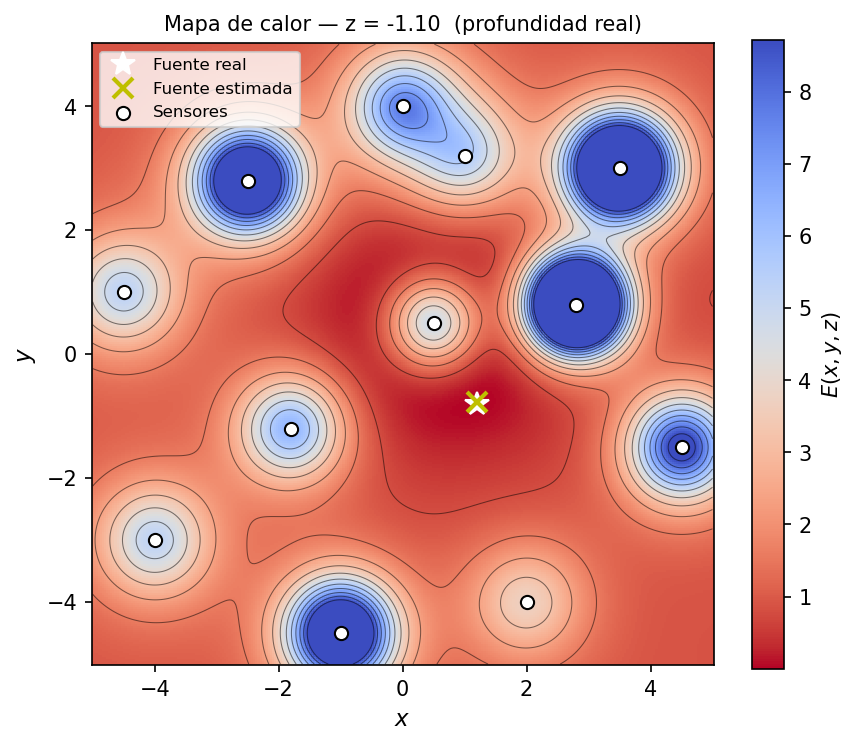
\includegraphics[width=0.95\textwidth]{Imagenes/corte_z_110.png}
        \end{block}

        \column{0.41\textwidth}

        \begin{block}{Interpretación}
            \scriptsize
            \begin{itemize}
                \item Corresponde exactamente a la \textbf{profundidad real} de la fuente simulada.
                \vspace{0.1cm}
                \item La región mínima se \textbf{concentra} claramente alrededor de $(x_{\text{real}},\ y_{\text{real}}) = (1.2,\ -0.8)$ km.
                \vspace{0.1cm}
                \item Las curvas de nivel forman anillos cerrados alrededor del mínimo.
            \end{itemize}
        \end{block}

        \vspace{0.2cm}

        \begin{exampleblock}{¿Qué nos dice?}
            \scriptsize
            El mínimo visual coincide con la \textbf{fuente real simulada}, validando que el modelo captura correctamente la señal sísmica.
        \end{exampleblock}

    \end{columns}

    \vspace{0.1cm}
    \begin{center}
        \footnotesize
        \textbf{Este es el corte más importante: el modelo reproduce mejor las observaciones aquí.}
    \end{center}

\end{frame}

% -----------------------------------------------
% FRAME 30c: z = -1.14  |  Diapositiva 35 → David
% -----------------------------------------------
% David
\begin{frame}{Mapa de Calor: Corte en $z = -1.14$ km — Corte Intermedio}

    \begin{columns}[T]

        \column{0.55\textwidth}

        \begin{block}{Corte en $z = -1.14$ km}
            \centering
            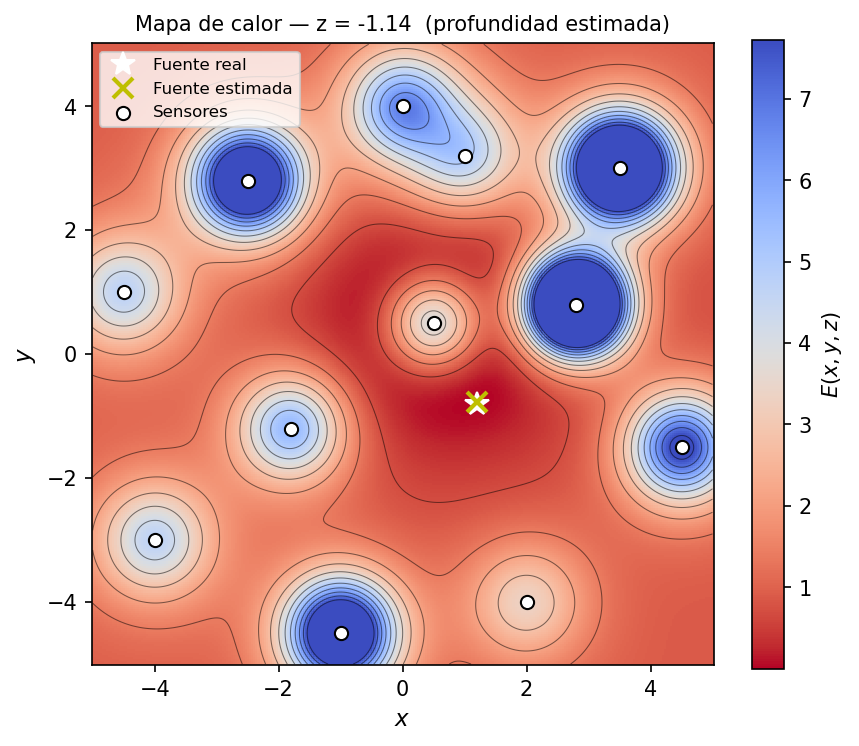
\includegraphics[width=0.95\textwidth]{Imagenes/corte_z_114.png}
        \end{block}

        \column{0.41\textwidth}

        \begin{block}{Interpretación}
            \scriptsize
            \begin{itemize}
                \item Corte \textbf{intermedio} entre $z_{\text{real}} = -1.10$ km y $z_{opt} = -1.22$ km.
                \vspace{0.1cm}
                \item La región mínima sigue \textbf{bien definida} y cercana a la fuente real.
                \vspace{0.1cm}
                \item Confirma la \textbf{estabilidad} del modelo ante pequeñas variaciones de $z$.
            \end{itemize}
        \end{block}

        \vspace{0.2cm}

        \begin{exampleblock}{¿Qué nos dice?}
            \scriptsize
            La región de bajo error se mantiene cerca de $(x_{\text{real}}, y_{\text{real}})$, confirmando la robustez de la solución de Gauss-Newton.
        \end{exampleblock}

    \end{columns}

    \vspace{0.1cm}
    \begin{center}
        \footnotesize
        \textbf{Pequeñas variaciones en $z$ desplazan levemente el mínimo pero no lo destruyen.}
    \end{center}

\end{frame}

% -----------------------------------------------
% FRAME 30d: z = -1.70  |  Diapositiva 36 → Danilo
% -----------------------------------------------
% Danilo
\begin{frame}{Mapa de Calor: Corte en $z = -1.70$ km — Plano Profundo}

    \begin{columns}[T]

        \column{0.55\textwidth}

        \begin{block}{Corte en $z = -1.70$ km}
            \centering
            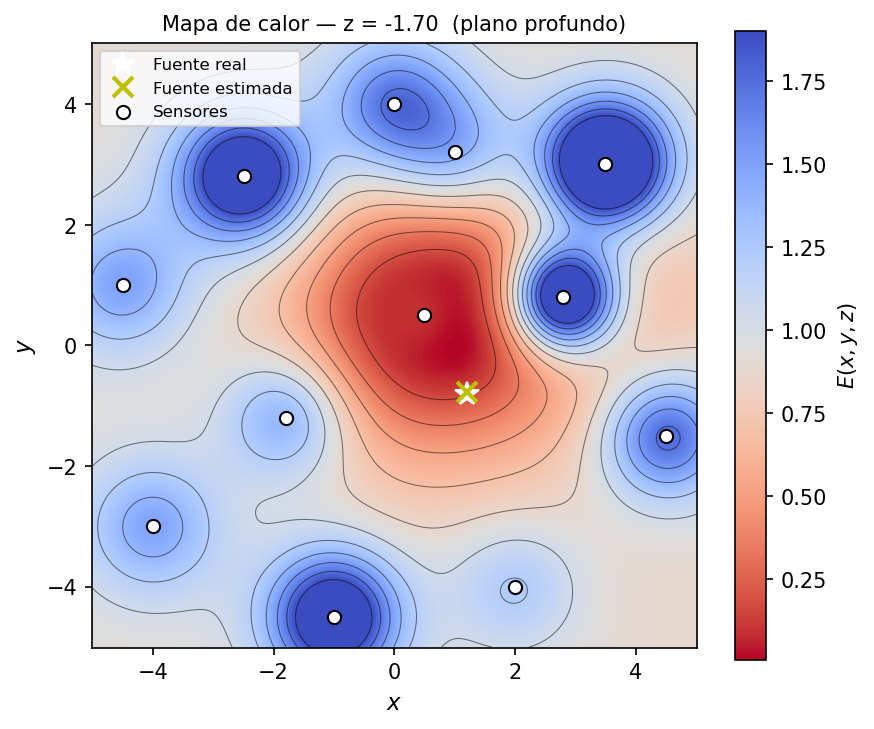
\includegraphics[width=0.95\textwidth]{Imagenes/corte_z_170.png}
        \end{block}

        \column{0.41\textwidth}

        \begin{block}{Interpretación}
            \scriptsize
            \begin{itemize}
                \item Este plano está \textbf{por debajo} de $z_{\text{real}}$ y $z_{opt}$.
                \vspace{0.1cm}
                \item La región mínima se \textbf{aleja y dispersa} respecto a los cortes anteriores.
                \vspace{0.1cm}
                \item El error mínimo en este plano es \textbf{mayor} que en $z_{\text{real}} = -1.10$ km.
            \end{itemize}
        \end{block}

        \vspace{0.2cm}

        \begin{exampleblock}{Conclusión Comparativa}
            \scriptsize
            Al alejarnos de la profundidad real, la función de error \textbf{pierde definición}, confirmando que $z_{\text{real}} = -1.10$ km es la profundidad que mejor explica las observaciones.
        \end{exampleblock}

    \end{columns}

    \vspace{0.1cm}
    \begin{center}
        \footnotesize
        \textbf{Comparar los 4 cortes revela la sensibilidad del modelo ante cambios de profundidad.}
    \end{center}

\end{frame}

% Diapositiva 37

% David
%=============================================
% Punto 11: Gráfica Emin(z) — mejor error posible para cada profundidad.
%=============================================

\begin{frame}{Análisis de Profundidad: Gráfica $E_{\min}(z)$}

    \begin{columns}[T]

        \column{0.52\textwidth}

        \begin{block}{$E_{\min}(z)$: Valor mínimo del error por profundidad}
            \centering
            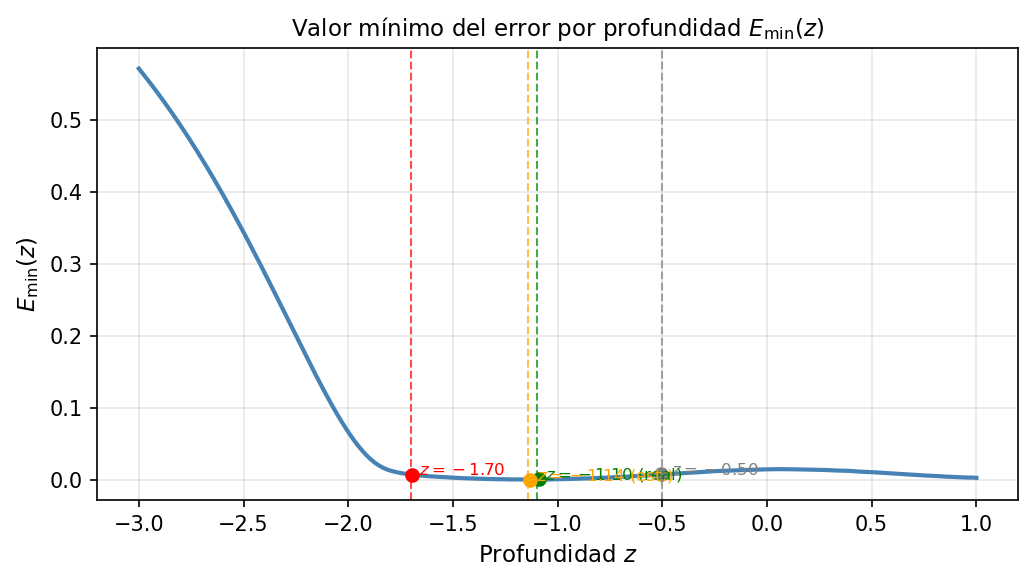
\includegraphics[width=0.95\textwidth]{Imagenes/emin_z.png}
        \end{block}

        \column{0.44\textwidth}

        \begin{block}{¿Qué representa esta gráfica?}
            \scriptsize
            \begin{itemize}
                \item Para cada $z$ se minimiza $E$ sobre $(x, y, A_0)$, obteniendo el \textbf{mejor ajuste posible} en ese plano.
                \vspace{0.15cm}
                \item La curva muestra \textbf{cómo varía la calidad del ajuste} según la profundidad.
                \vspace{0.15cm}
                \item El \textbf{mínimo global} $z_{opt} \approx -1.22$ km identifica la profundidad estimada del hipocentro.
            \end{itemize}
        \end{block}

        \vspace{0.2cm}

        \begin{exampleblock}{Interpretación Física}
            \scriptsize
            \begin{itemize}
                \item $z_{opt} \approx -1.22$ km con $E_{\min} \approx 8.50 \times 10^{-6}$
                \vspace{0.1cm}
                \item Diferencia con $z_{\text{real}} = -1.10$ km: solo \textbf{0.12 km}
                \vspace{0.1cm}
                \item La curvatura pronunciada indica \textbf{alta sensibilidad} del modelo a la profundidad.
            \end{itemize}
        \end{exampleblock}

    \end{columns}

    \vspace{0.15cm}
    \begin{center}
        \footnotesize
        \textbf{$E_{\min}(z)$ convierte el análisis 4D en una búsqueda unidimensional interpretable.}
    \end{center}

\end{frame}
% David
%=============================================
% Puntos 12-17: Trayectoria del mínimo, interpretación geométrica,
% relación visualización-optimización, región mínima,
% relación con fuente real y conclusión visual.
%=============================================

\begin{frame}{Interpretación Geométrica y Conclusión Visual}

    \begin{columns}[T]

        %===========================================
        % COLUMNA IZQUIERDA: Trayectoria del mínimo
        %===========================================
        \column{0.52\textwidth}

        \begin{block}{Trayectoria del mínimo en el plano $(x,y)$}
            \centering
            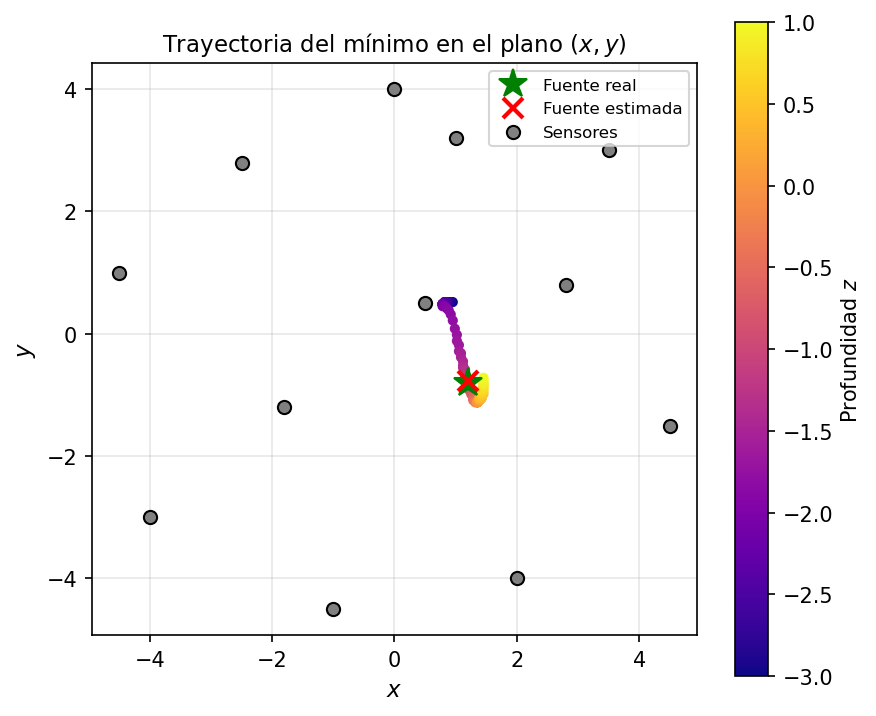
\includegraphics[width=0.92\textwidth]{Imagenes/trayectoria_minimo.png}
        \end{block}

        \vspace{0.1cm}
        \begin{center}
            \tiny \textcolor{gray}{Evolución de la posición del mínimo al variar la profundidad $z$.}
        \end{center}

        %===========================================
        % COLUMNA DERECHA: Interpretación y conclusión
        %===========================================
        \column{0.44\textwidth}

        \begin{block}{Interpretación Geométrica}
            \scriptsize
            \begin{itemize}
                \item La trayectoria muestra \textbf{cómo se desplaza} la ubicación estimada de la fuente al modificar $z$.
                \vspace{0.1cm}
                \item Las visualizaciones revelan la \textbf{forma de la superficie de error} y cómo el algoritmo converge hacia el mínimo.
                \vspace{0.1cm}
                \item La región mínima es la zona donde $A_{pred,i} \approx A_{obs,i}$ de manera más consistente.
            \end{itemize}
        \end{block}

        \vspace{0.2cm}

        \begin{exampleblock}{Relación con la Fuente Real}
            \scriptsize
            \begin{itemize}
                \item Las regiones de \textbf{menor error coinciden} con la ubicación real de la fuente simulada.
                \vspace{0.1cm}
                \item La visualización \textbf{confirma gráficamente} lo encontrado por el optimizador numérico.
            \end{itemize}
        \end{exampleblock}

    \end{columns}

    \vspace{0.15cm}
    \begin{center}
        \footnotesize
        \textbf{La visualización permite comprender intuitivamente cómo la optimización localiza la fuente sísmica.}
    \end{center}

\end{frame}



\end{document}